\documentclass[
  bibliography=totoc,     % Literatur im Inhaltsverzeichnis
  captions=tableheading,  % Tabellenüberschriften
  titlepage=firstiscover, % Titelseite ist Deckblatt
]{scrartcl}

% LaTeX2e korrigieren.
\usepackage{fixltx2e}
% Warnung, falls nochmal kompiliert werden muss
\usepackage[aux]{rerunfilecheck}

% deutsche Spracheinstellungen
\usepackage{polyglossia}
\setmainlanguage{german}

% unverzichtbare Mathe-Befehle
\usepackage{amsmath}
% viele Mathe-Symbole
\usepackage{amssymb}
% Erweiterungen für amsmath
\usepackage{mathtools}

% Fonteinstellungen
\usepackage{fontspec}
\defaultfontfeatures{Ligatures=TeX}

\usepackage[
  math-style=ISO,    % \
  bold-style=ISO,    % |
  sans-style=italic, % | ISO-Standard folgen
  nabla=upright,     % |
  partial=upright,   % /
]{unicode-math}

\setmathfont{Latin Modern Math}
\setmathfont[range={\mathscr, \mathbfscr}]{XITS Math}
\setmathfont[range=\coloneq]{XITS Math}
\setmathfont[range=\propto]{XITS Math}
% make bar horizontal, use \hslash for slashed h
\let\hbar\relax
\DeclareMathSymbol{\hbar}{\mathord}{AMSb}{"7E}
\DeclareMathSymbol{ℏ}{\mathord}{AMSb}{"7E}

% richtige Anführungszeichen
\usepackage[autostyle]{csquotes}

% Zahlen und Einheiten
\usepackage[
  locale=DE,                   % deutsche Einstellungen
  separate-uncertainty=true,   % Immer Fehler mit \pm
  per-mode=symbol-or-fraction, % m/s im Text, sonst Brüche
]{siunitx}

% chemische Formeln
\usepackage[version=3]{mhchem}

% schöne Brüche im Text
\usepackage{xfrac}

% Floats innerhalb einer Section halten
\usepackage[section, below]{placeins}
% Captions schöner machen.
\usepackage[
  labelfont=bf,        % Tabelle x: Abbildung y: ist jetzt fett
  font=small,          % Schrift etwas kleiner als Dokument
  width=0.9\textwidth, % maximale Breite einer Caption schmaler
]{caption}
% subfigure, subtable, subref
\usepackage{subcaption}

% Grafiken können eingebunden werden
\usepackage{graphicx}
% größere Variation von Dateinamen möglich
\usepackage{grffile}

% Standardplatzierung für Floats einstellen
\usepackage{float}
\floatplacement{figure}{htbp}
\floatplacement{table}{htbp}

% schöne Tabellen
\usepackage{booktabs}

% Seite drehen für breite Tabellen
\usepackage{pdflscape}

% Literaturverzeichnis
\usepackage{biblatex}
% Quellendatenbank
\addbibresource{lit.bib}
\addbibresource{programme.bib}

% Hyperlinks im Dokument
\usepackage[
  unicode,
  pdfusetitle,    % Titel, Autoren und Datum als PDF-Attribute
  pdfcreator={},  % PDF-Attribute säubern
  pdfproducer={}, % "
]{hyperref}
% erweiterte Bookmarks im PDF
\usepackage{bookmark}

% Trennung von Wörtern mit Strichen
\usepackage[shortcuts]{extdash}

\author{
  AUTOR A%
  \texorpdfstring{
    \\
    \href{mailto:authorA@udo.edu}{authorA@udo.edu}
  }{}%
  \texorpdfstring{\and}{, }
  AUTOR B
  \texorpdfstring{
    \\
    \href{mailto:authorB@udo.edu}{authorB@udo.edu}
  }{}
}
\publishers{TU Dortmund – Fakultät Physik}


\title[\LaTeX]{Verfassen wissenschaftlicher Texte mit \LaTeX}
\titlegraphic{figures/latex-vs-word.pdf}

\addbibresource{examples.bib}

\begin{document}

{
  \setbeamertemplate{footline}{}
  \begin{frame}
    \titlepage
  \end{frame}

  \begin{frame}[fragile]
    \centering
    {\Huge \LaTeX:}

    \vspace{10pt}
    \centering
    \begin{BVerbatim}[gobble=4]
    \DeclareRobustCommand{\LaTeX}{%
      L\kern-.36em%
      {\sbox\z@ T%
        \vbox to\ht\z@{\hbox{%
          \check@mathfonts
          \fontsize\sf@size\z@
          \math@fontsfalse\selectfont A}%
          \vss}%
      }%
      \kern-.15em%
      \TeX}
    \end{BVerbatim}

    \begin{center}
      \Huge
      … alles klar?
    \end{center}
\end{frame}
}

\begin{frame}{Übersicht}
  \tableofcontents
\end{frame}

\section{Umfrage}

\begin{frame}{Betriebssystem}
  \centering
  \includegraphics[height=0.9\textheight]{figures/os.pdf}
\end{frame}

\begin{frame}{Erfahrung mit LaTeX}
  \centering
  \includegraphics[height=0.9\textheight]{figures/experience.pdf}
\end{frame}

\section{Einführung}

\begin{frame}{Was ist \LaTeX?}
  \Large
  \linespread{1.5}
  \begin{itemize}
    \item \emph{Programmiersprache} zum Setzen von Text
    \item Markup $\Rightarrow$ kein
      \textcolor{vertexDarkRed}{W}hat-\textcolor{vertexDarkRed}{Y}ou-\textcolor{vertexDarkRed}{S}ee-\textcolor{vertexDarkRed}{I}s-\textcolor{vertexDarkRed}{W}hat-\textcolor{vertexDarkRed}{Y}ou-\textcolor{vertexDarkRed}{G}et

    \item \LaTeX-Code → Kompiler → Ausgabedokument (meist PDF)
    \item Open-Source, große Erweiterungsmöglichkeit (Pakete)
    \item Standard-Werkzeug in der Wissenschaft
  \end{itemize}
  \linespread{1.0}
\end{frame}

\begin{frame}{Warum \LaTeX?}
  \Large
  \linespread{1.5}
  \begin{itemize}
    \item Hervorragender Text- und Formelsatz
    \item Automatisierte Erstellung von Inhalts- und Literaturverzeichnis
    \item \TeX-Dateien sind reine Text-Dateien \\
      $\Rightarrow$ Gut für Versionskontrolle geeignet
    \item Sehr gute Vorlagen für wissenschaftliches Arbeiten
  \end{itemize}
  \linespread{1.0}
\end{frame}

\begin{frame}{Warum \LaTeX?}
  \Large
  \linespread{1.5}
  \begin{itemize}
    \item Ausgezeichnete Dokumentation
    \item Erweiterbar durch zahlreiche und mächtige Pakete
    \item Auf allen geläufigen Betriebssystemen verfügbar
    \item Ausgabe direkt als PDF mit Hyperlinks
  \end{itemize}
  \linespread{1.0}
\end{frame}

\begin{frame}{Geschichte}
  \begin{columns}
    \begin{column}{0.73\textwidth}
      \TeX:
      \begin{itemize}
        \item Geschrieben von Donald E. Knuth 1978, um sein Buch \enquote{The Art of Computer Programming} zu setzen
        \item Auf Aussprache achten!
        \item Version (2014): $3.14159265 → \symup{π}$
        \item Viele Erweiterungen: \eTeX, pdf\TeX, \XeTeX, \LuaTeX
      \end{itemize}

      \vspace{10pt}
      \LaTeX:
      \begin{itemize}
        \item Geschrieben von Leslie Lamport 1984
        \item Version (1994): \LaTeXe
        \item \LaTeX3 seit Anfang der Neunziger in Arbeit…
      \end{itemize}
    \end{column}
    \begin{column}{0.23\textwidth}
      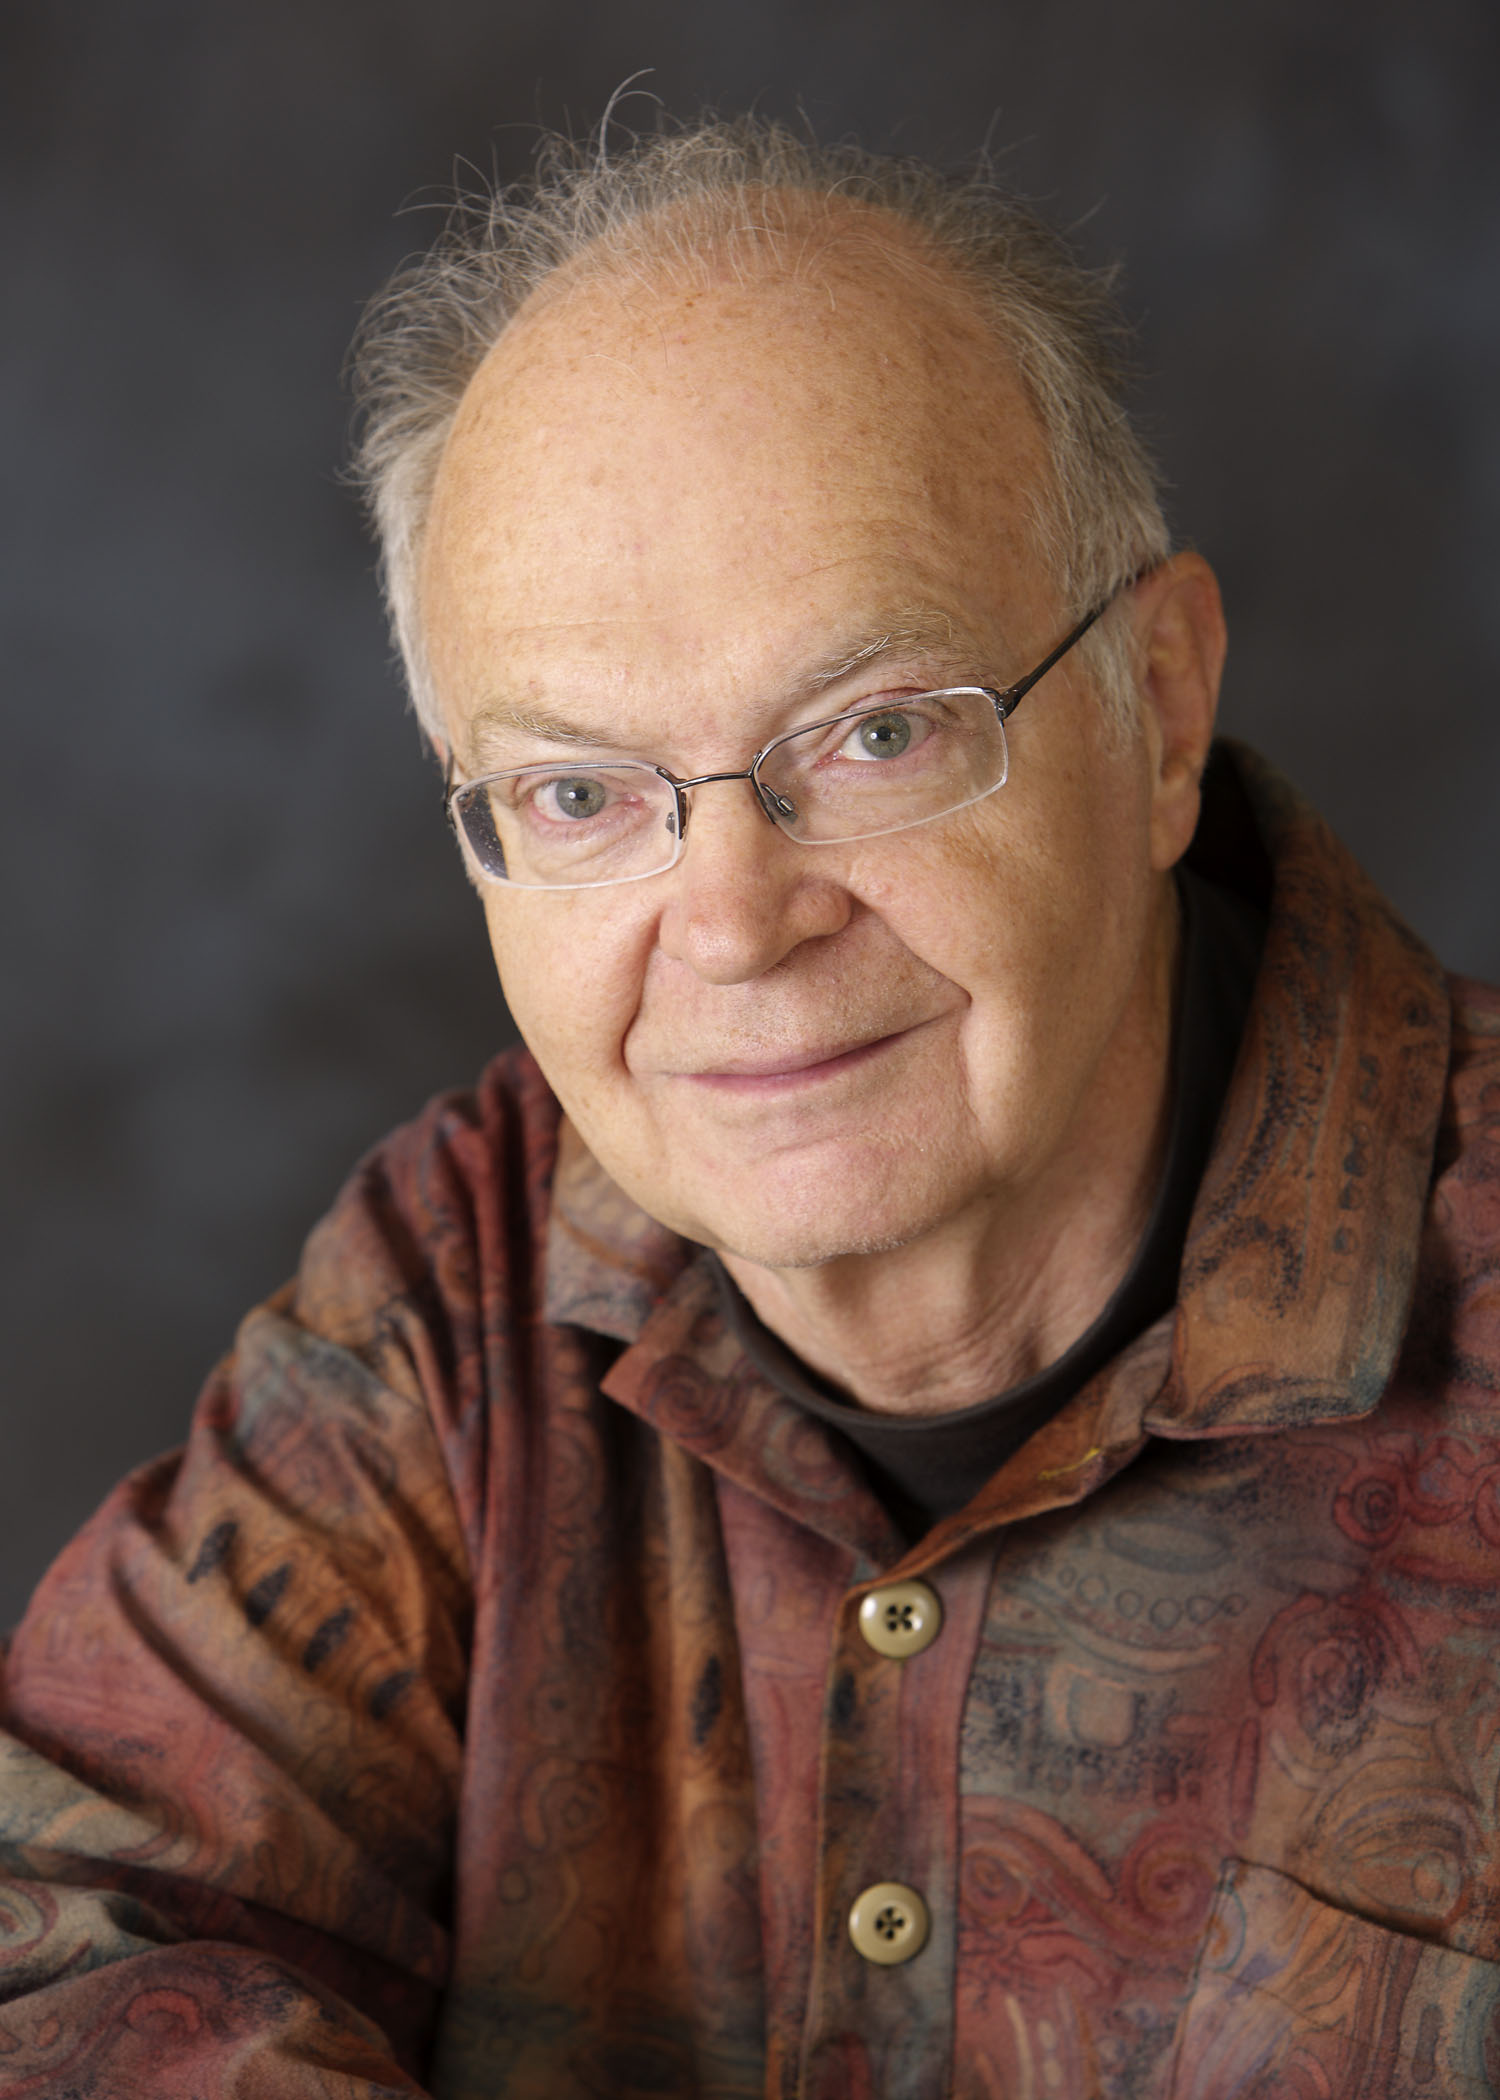
\includegraphics[height=0.45\textheight]{figures/knuth.jpg}\\
      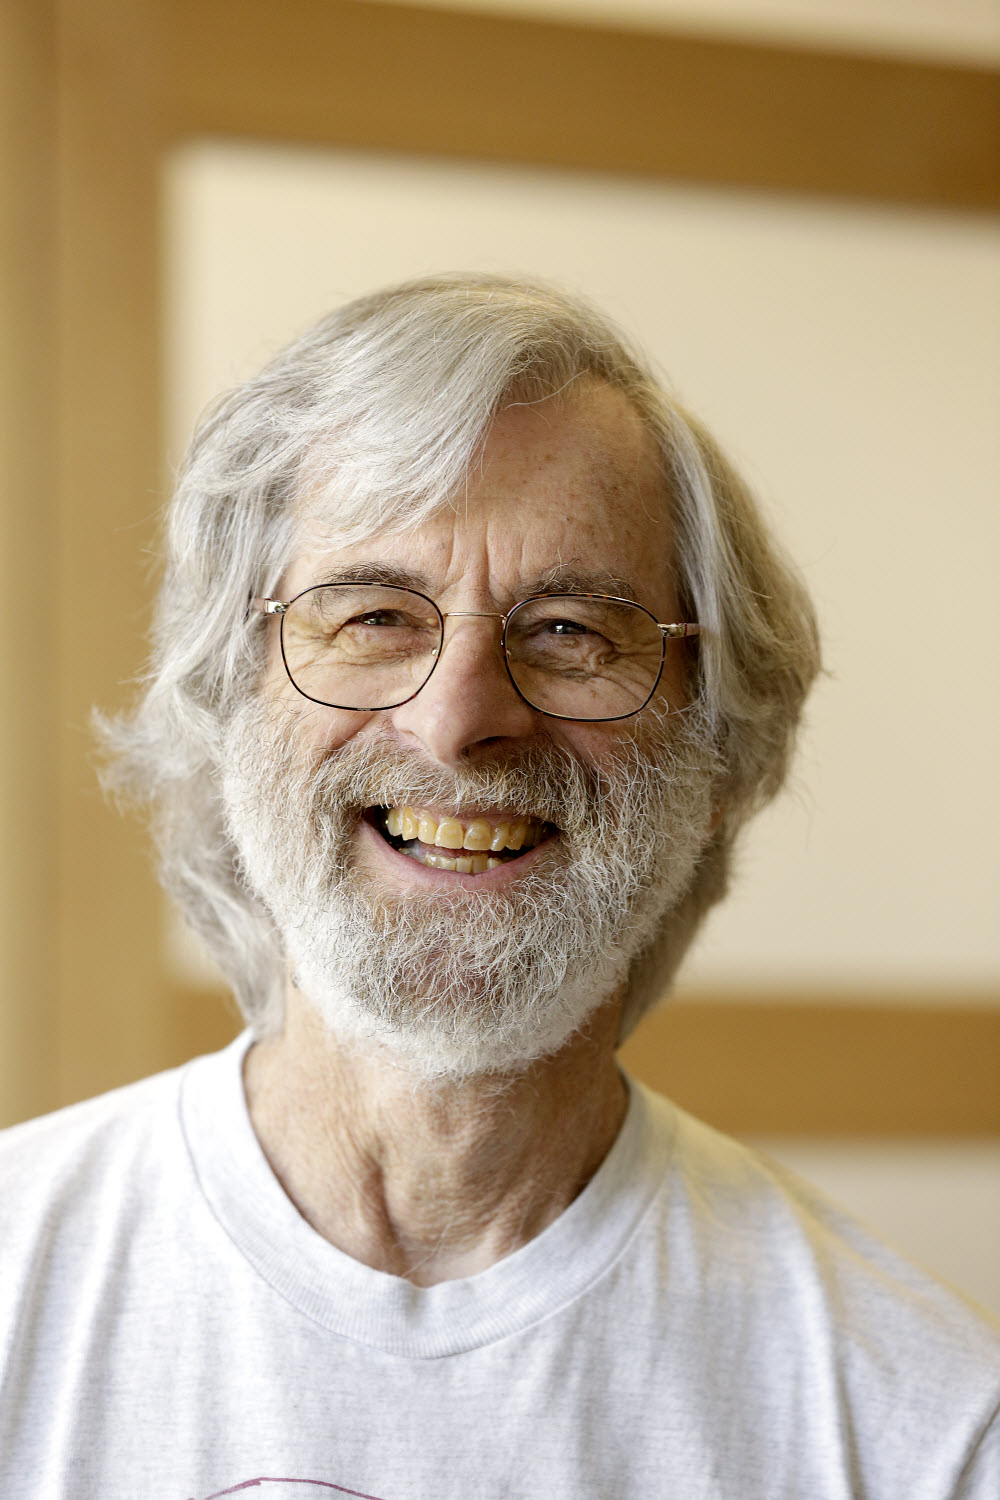
\includegraphics[height=0.45\textheight]{figures/lamport.jpg}
    \end{column}
  \end{columns}
\end{frame}

\begin{frame}{Dieser Kurs}
  \Large
  \linespread{1.5}
  \begin{itemize}
    \item In \LaTeX\ gibt es immer viele Möglichkeiten, ein Ziel zu erreichen
    \item Wir zeigen einen modernen Ansatz
    \item Wir erklären, warum wir diesen Ansatz gewählt haben
    \item Weitere Ansätze werden an manchen Stellen kurz erwähnt
  \end{itemize}
  \linespread{1.0}
\end{frame}

\begin{frame}{Begriffe}
  \Large
  \begin{description}
    \item[\TeX-Engine] Implementierung von \TeX, wird als Programm ausgeführt
    \item[\TeX-Format] Paket, welches standardmäßig geladen wird, z.B. \LaTeX
  \end{description}

  \vspace{10pt}
  Eine Kombination davon ist oft ein neues Programm.\\[10pt]
  Beispiel: \texttt{dvilualatex} = \LuaTeX\ + \LaTeX\ + DVI-Output (statt PDF)
\end{frame}

\section{Grundlagen}

\begin{frame}[fragile]{Das Dokument}
  Diese drei Zeilen braucht jedes \LaTeX-Dokument:
  \begin{columns}[onlytextwidth, t]
    \begin{column}{0.50\textwidth}
      \begin{block}{Code}
        \begin{lstlisting}
          \documentclass[optionen]{klasse}
            % .
            % Präambel
            % .
            % .
          \begin{document}
            % Inhalt des Dokuments
          \end{document}
        \end{lstlisting}
      \end{block}
    \end{column}
    \begin{column}{0.48\textwidth}
      \begin{block}{\lstinline+\\documentclass+}
        Vorlage wählen, mit Optionen anpassen.
      \end{block}
      \begin{block}{Präambel}
        Globale Optionen und zusätzliche Pakete.
      \end{block}
      \begin{block}{\texttt{document}-Umgebung}
        Inhalt des Dokuments.
      \end{block}
    \end{column}
  \end{columns}
\end{frame}
\begin{frame}[fragile]{Hallo Welt}
  \begin{CodeExample}{0.5}
    \begin{lstlisting}
      \documentclass{scrartcl}
      \begin{document}
        Hallo Welt!
      \end{document}
    \end{lstlisting}
  \CodeResult
    \begin{minipage}[c][4\baselineskip][c]{\textwidth}
      \strut
      Hallo Welt!
    \end{minipage}
  \end{CodeExample}
\end{frame}

\begin{frame}[fragile]{Syntax: Befehle}
  \LaTeX-Befehle beginnen stets mit einem \verb+\+ (Backslash).

  Obligatorische Argumente stehen in \lstinline+{ }+, optionale Argumente stehen in \lstinline+[ ]+.
    \begin{block}{Syntax}
      \begin{lstlisting}
        \befehl[optional]{obligatorisch}
        \befehl*[optional]{obligatorisch}
      \end{lstlisting}
    \end{block}

  \verb+*+ ruft häufig eine Alternativform des Befehls auf.
  \begin{CodeExplanation}{0.53}[Code][Erklärung]
    \begin{lstlisting}
      \documentclass[paper=a4]{scrartcl}

      \tableofcontents
      \frac{1}{2}
      % Kommentar
    \end{lstlisting}
  \Explanation
    \strut
    Dokumentenklasse \texttt{scrartcl},\\
    Papierformat DIN\,A4 \\
    Keine Argumente \\
    Zwei oder mehr Pflichtargumente\\
    \verb+%+-Zeichen für Kommentare
  \end{CodeExplanation}
\end{frame}

\begin{frame}[fragile]{Syntax: Umgebungen}
  \begin{itemize}
    \item Einstellungen für Bereich des Dokuments
    \item Extrem vielseitig
    \item Können ggfs.\ auch Optionen übergeben bekommen
    \item Oft auch Alternativform mit \lstinline+*+
  \end{itemize}
  \begin{CodeExplanation}{0.65}[Syntax][Beispiel]
    \begin{lstlisting}
      \begin{Umgebung}[optional]{obligatorisch}
        % .
      \end{Umgebung}
    \end{lstlisting}
    \Explanation
    \begin{lstlisting}
      \begin{flushright}
        % .
      \end{flushright}
    \end{lstlisting}
  \end{CodeExplanation}
\end{frame}

\begin{frame}[fragile]{Syntax: Umgebungen}
  \begin{itemize}
    \item Können weitere Umgebungen enthalten
    \item Diese müssen aber in der Umgebung wieder geschlossen werden
  \end{itemize}
  \begin{columns}[onlytextwidth, t]
    \begin{column}{0.48\textwidth}
      \begin{block}{Geht:}
        \begin{lstlisting}
          \begin{document}
            \begin{flushright}
              % .
            \end{flushright}
          \end{document}
        \end{lstlisting}
      \end{block}
    \end{column}
    \begin{column}{0.48\textwidth}
      \begin{alertblock}{Geht nicht:}
        \begin{lstlisting}
          \begin{itemize}
            \begin{enumerate}
              % .
          \end{itemize}
            \end{enumerate}
        \end{lstlisting}
      \end{alertblock}
    \end{column}
  \end{columns}
\end{frame}

\begin{frame}[fragile]{Standardpakete}
  Die hier aufgezählten Pakete sollten immer geladen werden, da sie wesentliche Funktionen bieten und wichtige Einstellungen vornehmen.
  \vspace{-1em}
  \begin{CodeExplanation}{0.52}[Paket][Funktion]
    \begin{lstlisting}
      \usepackage[aux]{rerunfilecheck}


      \usepackage{polyglossia}
      \setmainlanguage{german}
      \usepackage{fontspec}

      % mehr Pakete hier

      \usepackage[unicode]{hyperref}

      \usepackage{bookmark}
    \end{lstlisting}
  \Explanation
    \strut
    Warnung, falls nochmal kompiliert werden muss. \\[\baselineskip]
  Deutsche Spracheinstellungen. \\[\baselineskip]
    Für Fonteinstellungen \\[3\baselineskip]
    Für Hyperlinks (z.B. Inhaltsverzeichnis → Kapitel). \\
    Erweiterte Bookmarks im PDF.
  \end{CodeExplanation}
  Die Reihenfolge ist manchmal wichtig, z.B. damit Pakete die Spracheinstellung kennen.
\end{frame}

\begin{frame}[fragile]{
  KOMA-Script-Klassen
  \hfill
  \doc{http://mirrors.ctan.org/macros/latex/contrib/koma-script/doc/scrguide.pdf}{\textsf{KOMA-Skript}}
}
  \begin{itemize}
    \item \texttt{scrartcl}, \texttt{scrreprt} und \texttt{scrbook}
    \item Sehr gute Vorlagen
    \item Schnell global mit Klassenoptionen anpassbar
  \end{itemize}
  \begin{block}{Fürs Praktikum empfohlenene Klasse}
    \begin{lstlisting}
      \documentclass[…]{scrartcl}
    \end{lstlisting}
  \end{block}
\end{frame}

\begin{frame}[fragile]{
  Fonteinstellungen
  \hfill
  \doc{http://mirrors.ctan.org/macros/latex/contrib/fontspec/fontspec.pdf}{fontspec}
}
  Standardeinstellung sind die Latin-Modern-Fonts.
  \vspace{1em}
  \begin{CodeExplanation}{0.48}[Latin Modern][Alternativ zum Beispiel: Libertinus]
    \begin{lstlisting}
      \usepackage{fontspec}
    \end{lstlisting}
  \Explanation
    \begin{lstlisting}
      \usepackage{fontspec}
      \setmainfont{Libertinus Serif}
      \setsansfont{Libertinus Sans}
      \setmonofont{Libertinus Mono}
    \end{lstlisting}
  \end{CodeExplanation}
  \begin{itemize}
    \item Jede System-Schriftart kann genutzt werden
    \item \alert{Das ist i.A. nicht sinnvoll: \fontspec{Comic Sans MS} Hallo Welt in Comic Sans!}
    \item Schriften müssen zueinander passen
    \item Schriften müssen alle benötigten Sonderzeichen enthalten
    \item Bei Änderung auch Mathefont anpassen → später
    \item Welche Schriftarten zueinander passen ist eine Wissenschaft für sich.
  \end{itemize}
\end{frame}

\begin{frame}[fragile]{Gerüst}
  \begin{lstlisting}
    \documentclass{scrartcl}

    \usepackage[aux]{rerunfilecheck}

    \usepackage{fontspec}

    \usepackage{polyglossia}
    \setmainlanguage{german}

    % mehr Pakete hier

    \usepackage[unicode]{hyperref}
    \usepackage{bookmark}
    % Einstellungen hier, z.B. Fonts

    \begin{document}
      % Text hier
    \end{document}
  \end{lstlisting}
\end{frame}

\begin{frame}[fragile]{Das Ausgabedokument erstellen}
  Es gibt verschiedene \LaTeX-Kompiler, die verschiedene Ausgabeformate erzeugen können.
  Der modernste Kompiler, der PDF-Dateien erstellt, ist \alert{\texttt{lualatex}}.

  \begin{block}{\LaTeX-Dokument kompilieren}
    Terminal öffnen:
    \begin{lstlisting}
      lualatex MeinDokument.tex
    \end{lstlisting}
  \end{block}

  \begin{alertblock}{Vorsicht!}
    \begin{itemize}
      \item Es muss fast immer mindestens zweimal kompiliert werden.
      \item Es werden diverse Hilfs- und Logdateien erzeugt.
      \item Die Input-Dokumente müssen UTF-8 codiert sein.
    \end{itemize}
  \end{alertblock}
\end{frame}

\begin{frame}{\texttt{texdoc}}
  \LaTeX\ und (fast) alle Pakete sind hervorragend dokumentiert. Die Dokumentation wird automatisch mitinstalliert.
  \begin{block}{Dokumentation zu einem Paket}
    \texttt{texdoc \textit{paket}}
  \end{block}

  Dabei ist \texttt{\textit{paket}} ein Suchstring.
  \begin{block}{Nach Dokumentation suchen}
    \texttt{texdoc -l \textit{name}}
  \end{block}

  Es ist wichtig zu lernen, Dokumentationen zu lesen. Probiert es an den oben genannten Paketen aus.

  \vspace{10pt}
  Alternativ kann man das Paket bei Google suchen, dann findet man auch die Dokumentation auf CTAN.
\end{frame}

\section{Text erstellen}

\begin{frame}[fragile]{Text schreiben}
  \begin{block}{Beispiel}
    \begin{lstlisting}
      % Präambel
      \begin{document}
        Hallo, Welt!

        Dies ist ein dummer Beispieltext.
        Er soll zeigen, dass \LaTeX sich nicht um
        Zeilenumbrüche im Code    oder    zuviele
        Leerzeichen kümmert.

        Ein Absatz wird mit einer leeren Code-Zeile
        markiert.
      \end{document}
    \end{lstlisting}
  \end{block}
\end{frame}

\begin{frame}[fragile]{Konventionen für Text}
  \begin{itemize}
    \item Höchstens ein Satz pro Code-Zeile
    \item Absätze werden durch eine Leerzeile markiert
    \item Im Fließtext sollten keine Umbrüche mit \lstinline+\\+ erzwungen werden
  \end{itemize}
  \begin{alertblock}{Sonderzeichen}
    Viele Sonderzeichen sind \LaTeX-Steuerzeichen.
    Damit diese im Text genutzt werden können, muss meist ein \verb+\+ vorangestellt oder ein Befehl genutzt werden.
  \end{alertblock}
  \begin{CodeExample}{0.7}
    \begin{lstlisting}
      \# \$ \% \& \_ \{ \}
      \textbackslash \textasciicircum \textasciitilde
    \end{lstlisting}
  \CodeResult
    \strut
    \# \$ \% \& \_ \{ \} \\
    \textbackslash\ \textasciicircum\ \textasciitilde
  \end{CodeExample}
\end{frame}

\begin{frame}[fragile]{Textauszeichnung}
  Änderungen der Schrifteigenschaften sind mit diesen Befehlen möglich:
  \begin{CodeExample}{0.60}
    \begin{lstlisting}
      \textit{kursiv} \emph{kursiv}
      \textbf{fett}
      \textbf{\textit{fett-kursiv}}
      \textrm{Serifen-Schrift}
      \texttt{Mono-Schrift}
      \textsf{Sans-Serif-Schrift}
      \textsc{Kapitälchen}
    \end{lstlisting}
  \CodeResult
    \strut
    \textit{kursiv} \emph{kursiv} \\
    \textbf{fett} \\
    \textbf{\textit{fett-kursiv}} \\
    \textrm{Serifen-Schrift} \\
    \texttt{Mono-Schrift} \\
    \textsf{Sans-Serif-Schrift} \\
    \textsc{Kapitälchen}
  \end{CodeExample}

  \vspace{1em}
  Diese Befehle sollten sehr selten benutzt werden, semantischer Markup ist besser.
\end{frame}

\begin{frame}[fragile]{Schriftgrößen}
  Gelten immer für den aktuellen Block, z.\,B. in einer Umgebung oder zwischen \lstinline+{ }+
  \begin{CodeExample}{0.48}
    \begin{lstlisting}
      {\tiny tiny}
      {\small small}
      {\normalsize normal}
      {\large large}
      {\huge huge}
    \end{lstlisting}
  \CodeResult
    \begin{minipage}[c][5\baselineskip][c]{\textwidth}
      {\tiny tiny}
      {\small small}
      {\normalsize normal}
      {\large large}
      {\huge huge}
    \end{minipage}
  \end{CodeExample}
  \vspace{1em}
  \begin{block}{Alle Größen}
    \begin{lstlisting}
      \tiny, \scriptsize, \footnotesize, \small, \normalsize, \large, \Large, \LARGE, \huge, \Huge
    \end{lstlisting}
  \end{block}
  Auch diese Befehle sollten nur über semantischen Markup benutzt werden.
\end{frame}

\begin{frame}[fragile]{Inhalt auslagern}
  \begin{block}{Code}
    \begin{lstlisting}
      \documentclass[
  bibliography=totoc,     % Literatur im Inhaltsverzeichnis
  captions=tableheading,  % Tabellenüberschriften
  titlepage=firstiscover, % Titelseite ist Deckblatt
]{scrartcl}

% LaTeX2e korrigieren.
\usepackage{fixltx2e}
% Warnung, falls nochmal kompiliert werden muss
\usepackage[aux]{rerunfilecheck}

% deutsche Spracheinstellungen
\usepackage{polyglossia}
\setmainlanguage{german}

% unverzichtbare Mathe-Befehle
\usepackage{amsmath}
% viele Mathe-Symbole
\usepackage{amssymb}
% Erweiterungen für amsmath
\usepackage{mathtools}

% Fonteinstellungen
\usepackage{fontspec}
\defaultfontfeatures{Ligatures=TeX}

\usepackage[
  math-style=ISO,    % \
  bold-style=ISO,    % |
  sans-style=italic, % | ISO-Standard folgen
  nabla=upright,     % |
  partial=upright,   % /
]{unicode-math}

\setmathfont{Latin Modern Math}
\setmathfont[range={\mathscr, \mathbfscr}]{XITS Math}
\setmathfont[range=\coloneq]{XITS Math}
\setmathfont[range=\propto]{XITS Math}
% make bar horizontal, use \hslash for slashed h
\let\hbar\relax
\DeclareMathSymbol{\hbar}{\mathord}{AMSb}{"7E}
\DeclareMathSymbol{ℏ}{\mathord}{AMSb}{"7E}

% richtige Anführungszeichen
\usepackage[autostyle]{csquotes}

% Zahlen und Einheiten
\usepackage[
  locale=DE,                   % deutsche Einstellungen
  separate-uncertainty=true,   % Immer Fehler mit \pm
  per-mode=symbol-or-fraction, % m/s im Text, sonst Brüche
]{siunitx}

% chemische Formeln
\usepackage[version=3]{mhchem}

% schöne Brüche im Text
\usepackage{xfrac}

% Floats innerhalb einer Section halten
\usepackage[section, below]{placeins}
% Captions schöner machen.
\usepackage[
  labelfont=bf,        % Tabelle x: Abbildung y: ist jetzt fett
  font=small,          % Schrift etwas kleiner als Dokument
  width=0.9\textwidth, % maximale Breite einer Caption schmaler
]{caption}
% subfigure, subtable, subref
\usepackage{subcaption}

% Grafiken können eingebunden werden
\usepackage{graphicx}
% größere Variation von Dateinamen möglich
\usepackage{grffile}

% Standardplatzierung für Floats einstellen
\usepackage{float}
\floatplacement{figure}{htbp}
\floatplacement{table}{htbp}

% schöne Tabellen
\usepackage{booktabs}

% Seite drehen für breite Tabellen
\usepackage{pdflscape}

% Literaturverzeichnis
\usepackage{biblatex}
% Quellendatenbank
\addbibresource{lit.bib}
\addbibresource{programme.bib}

% Hyperlinks im Dokument
\usepackage[
  unicode,
  pdfusetitle,    % Titel, Autoren und Datum als PDF-Attribute
  pdfcreator={},  % PDF-Attribute säubern
  pdfproducer={}, % "
]{hyperref}
% erweiterte Bookmarks im PDF
\usepackage{bookmark}

% Trennung von Wörtern mit Strichen
\usepackage[shortcuts]{extdash}

\author{
  AUTOR A%
  \texorpdfstring{
    \\
    \href{mailto:authorA@udo.edu}{authorA@udo.edu}
  }{}%
  \texorpdfstring{\and}{, }
  AUTOR B
  \texorpdfstring{
    \\
    \href{mailto:authorB@udo.edu}{authorB@udo.edu}
  }{}
}
\publishers{TU Dortmund – Fakultät Physik}

      \begin{document}
        \input{Teil1.tex}
        \input{Teil2.tex}
        % .
      \end{document}
    \end{lstlisting}
  \end{block}
  \begin{itemize}
    \item Verschachtelung möglich
    \item Zur Aufteilung größerer Dokumente (z.B. diese Präsentation)
    \item Für häufig wiederverwendeten Code (Header, Erläuterungen zu Fehlerrechnung, …)
    \item Für per Skript erzeugte Tabelleninhalte
  \end{itemize}
\end{frame}

\begin{frame}[fragile]{
  Anführungszeichen
  \hfill\doc{http://mirrors.ctan.org/macros/latex/contrib/csquotes/csquotes.pdf}{csquotes}
}
  Die richtigen Anführungszeichen, wo die Satzzeichen hingehören und vieles mehr hängt von der Sprache ab.
  So macht man es richtig:
  \begin{Packages}
    \begin{lstlisting}
      \usepackage[autostyle]{csquotes}    % nach polyglossia
      \setotherlanguages{english, french} % andere Sprachen laden
    \end{lstlisting}
  \end{Packages}
  \begin{CodeExample}{0.60}
    \begin{lstlisting}
      foo \enquote{bar} baz
      \enquote{foo \enquote{bar} baz}
      \textenglish{\enquote{foo}}
      \textfrench{\enquote{foo}}
      \textcquote{root}{foo}
    \end{lstlisting}
  \CodeResult
    \strut
    foo \enquote{bar} baz \\
    \enquote{foo \enquote{bar} baz} \\
    \textenglish{\enquote{foo}} \\
    \textfrench{ \enquote{foo}} \\
    \textcquote{root}{foo}
    % work around polyglossia bug #68
    \directlua{polyglossia.desactivate_frpt()}
  \end{CodeExample}
\end{frame}

\section{Aufzählungen}

\begin{frame}[fragile]{Aufzählungen: Itemize}
  \LaTeX\ bietet verschiedene Umgebungen für Aufzählungen.
  Für unnummerierte Listen wird \texttt{itemize} genutzt.
  Wie alle anderen Umgebungen können diese auch verschachtelt werden.
  \begin{columns}[t]
    \begin{column}{0.47\textwidth}
      \begin{block}{\LaTeX-Code}
        \begin{lstverbatim}
        \begin{itemize}
          \item Punkt 1
          \item Punkt 2
            \begin{itemize}
              \item Unterpunkt 1
              \item Unterpunkt 2
            \end{itemize}
          \item[→] Punkt 3
        \end{itemize}
        \end{lstverbatim}
      \end{block}
    \end{column}
    \begin{column}{0.47\textwidth}
      \begin{block}{Ergebnis}
        \begin{itemize}
          \item Punkt 1
          \item Punkt 2
            \begin{itemize}
              \item Unterpunkt 1
              \item Unterpunkt 2
            \end{itemize}
          \item[→] Punkt 3
        \end{itemize}
      \end{block}
    \end{column}
  \end{columns}
\end{frame}

\begin{frame}[fragile]{Aufzählungen: Enumerate}
  Für nummerierte Listen wird \texttt{enumerate} genutzt.
  \begin{columns}[t]
    \begin{column}{0.47\textwidth}
      \begin{block}{\LaTeX-Code}
        \begin{lstverbatim}
        \begin{enumerate}
          \item Punkt 1
          \item Punkt 2
            \begin{enumerate}[(a)]
              \item Unterpunkt 1
              \item Unterpunkt 2
            \end{enumerate}
          \item Punkt 3
        \end{enumerate}
        \end{lstverbatim}
      \end{block}
    \end{column}
    \begin{column}{0.47\textwidth}
      \begin{block}{Ergebnis}
        \begin{enumerate}
          \item Punkt 1
          \item Punkt 2
            \begin{enumerate}
              \item Unterpunkt 1
              \item Unterpunkt 2
            \end{enumerate}
          \item Punkt 3
        \end{enumerate}
      \end{block}
      Anpassung der Listen mit dem Paket \texttt{enumitem}
    \end{column}
  \end{columns}
\end{frame}

\begin{frame}[fragile]{Aufzählungen: Description}
  Zur Beschreibung von Stichwörtern wird \texttt{description} benutzt, dabei wird das
Stichwort \verb-\item- als optionales Argument übergeben.
  \begin{columns}[t]
    \begin{column}{0.47\textwidth}
      \begin{block}{\LaTeX-Code}
        \begin{lstverbatim}
        \begin{description}
          \item[\LaTeX] gut
          \item[Word] böse
        \end{description}
        \end{lstverbatim}
      \end{block}
    \end{column}
    \begin{column}{0.47\textwidth}
      \begin{block}{Ergebnis}
        \begin{description}
          \item[\LaTeX] gut
          \item[Word] böse
        \end{description}
      \end{block}
    \end{column}
  \end{columns}
\end{frame}

\section{Struktur}

\begin{frame}[fragile]{Titelseite und Metadaten}
  \LaTeX\ erstellt automatisch eine Titelei aus den Metadaten. \\
  Mit der Klassenoption \lstinline{titlepage=firstiscover} wird diese  als eigene Seite gesetzt.
  
  \begin{block}{Neue Klassenoption}
    \begin{lstlisting}
      \documentclass[…, titlepage=firstiscover, …]{scrartcl}
    \end{lstlisting}
  \end{block}

  \begin{block}{Empfehlung fürs Praktikum:}
    \begin{lstlisting}
      \title{101 Titel des Versuchs}
      % Mehrere Autoren mit \and:
      \author{Max Mustermann \and Maria Musterfrau}
      \date{Durchführung: 26.09.2014, Abgabe: 29.09.2014}
    \end{lstlisting}
  \end{block}

  \begin{block}{Titelseite generieren}
    \begin{lstlisting}
      \maketitle
    \end{lstlisting}
  \end{block}
\end{frame}

\begin{frame}[fragile]{Gliederung}
  \LaTeX\ bietet Befehle zum erstellen von Gliederungsebenen.
  Diese werden automatisch nummeriert und in entsprechend größerer und fetter Schrift gesetzt.

  \begin{block}{Gliederungsebenen für \texttt{scrartcl}}
    \begin{lstlisting}
      \section{Überschrift}
      \subsection{Überschrift}
      \subsubsection{Überschrift}
      \paragraph{Überschrift}    % wird nicht nummeriert
      \subparagraph{Überschrift} % wird nicht nummeriert
    \end{lstlisting}
  \end{block}
  \begin{block}{Höhere Gliederungsebenen für \texttt{scrreprt} und \texttt{scrbook}}
    \begin{lstlisting}
      \part{Überschrift}
      \chapter{Überschrift}
      \section{Überschrift}
    \end{lstlisting}
  \end{block}
\end{frame}

\begin{frame}[fragile]{Inhaltsverzeichnis}
  Aus den Gliederungselementen kann automatisch das Inhaltsverzeichnis erzeugt werden.
  \begin{block}{Inhaltsverzeichnis generieren}
    \begin{lstlisting}
      \tableofcontents
      \newpage
    \end{lstlisting}
  \end{block}
\end{frame}

\begin{frame}[fragile]{Referenzen}
  \begin{block}{Code}
    \begin{lstlisting}
      \section{Messung mit Apparatur 2}
      \label{sec:apparatur2}
      % .
      \section{Auswertung}
      Wie in \ref{sec:apparatur2} beschrieben, ...
    \end{lstlisting}
  \end{block}
  \begin{itemize}
    \item Auch für Gleichungen, Grafiken, Tabellen → später
    \item Für Übersichtlichkeit sollten Labels den Typ der Referenz nennen:
      \begin{description}
        \item[Sections]    \texttt{sec:}
        \item[Gleichungen] \texttt{eqn:}
        \item[Abbildungen] \texttt{fig:}
        \item[Tabellen]    \texttt{tab:}
      \end{description}
    \item Bei Gleichungen: \lstinline+\eqref+ (\texttt{amsmath} laden) statt \lstinline+\ref+ → setzt Klammern: \eqref{eqn:maxwell1}
    \item \lstinline+\label+ immer nach dem, worauf verwiesen wird
  \end{itemize}
\end{frame}

\section{Zahlen und Einheiten}

\begin{frame}[fragile]{Zahlen und Einheiten}
  \begin{itemize}
    \item Regeln zur Benutzung der SI-Einheiten: \\
      \url{http://www.bipm.org/utils/common/pdf/si_brochure_8_en.pdf}
    \item Einheiten werden aufrecht gesetzt
    \item Zwischen Zahl und Einheit steht ein kleines Leerzeichen
    \item Ab 5 Stellen wird ein kleines Leerzeichen als 1000er Trennzeichen genutzt:
  \end{itemize}

  \begin{CodeExample}{0.7}[Zahl mit Einheit]
    \begin{lstlisting}
      $5\,\mathrm{kg}$
    \end{lstlisting}
    \CodeResult
    $5\,\mathrm{kg}$
  \end{CodeExample}
  \begin{CodeExample}{0.7}[Zahl mit mehr als vier Stellen]
    \begin{lstlisting}
      $10\,000$
    \end{lstlisting}
    \CodeResult
    $10\,000$
  \end{CodeExample}
  \begin{CodeExample}{0.7}[Zehnerpotenz mit Unsicherheit in Klammern]
    \begin{lstlisting}
      $(5{,}34 \pm 0{,}54) \cdot 10^{-3}\,\mathrm{GeV}$
    \end{lstlisting}
    \CodeResult
    $(5{,}34 \pm 0{,}54) \cdot 10^{-3}\,\mathrm{GeV}$
  \end{CodeExample}
  
  \onslide<2->{%
  \begin{center}
    \LARGE  Das muss einfacher gehen
  \end{center}
  }
\end{frame}

\begin{frame}[fragile]{
  Das \texttt{siunitx}-Paket
  \hfill
  \doc{http://mirrors.ctan.org/macros/latex/contrib/siunitx/siunitx.pdf}{siunitx}
}
\begin{itemize}
    \item \texttt{siunitx} stellt Befehle zur Verfügung, die das korrekte Setzen von Zahlen und Einheiten stark vereinfachen
    \item Funktioniert in Fließtext und Matheumgebung
    \item[$\color{vertexDarkRed}\Rightarrow$] Dieses Paket sollte \alert{immer} und für \alert{jede} Zahl mit oder ohne Einheit verwendet werden.
\end{itemize}
  \begin{Packages}
    \begin{lstlisting}
      \usepackage[
        locale=DE,
        separate-uncertainty=true,  % Immer Fehler mit ±
        per-mode=symbol-or-fraction, % m/s im Text, sonst \frac
        % alternativ:
        % per-mode=reciprocal,      % m s^{-1}
        % output-decimal-marker=.,         % . statt , für Dezimalzahlen
      ]{siunitx}
    \end{lstlisting}
  \end{Packages}
\end{frame}

\begin{frame}[fragile]{\texttt{siunitx}: Zahlen mit \lstinline+\\num+}
  \begin{CodeExample}{0.7}[Zahlen mit automatischen 3er-Gruppen]
    \begin{lstlisting}
      \num{1.23456}
      \num{987654321}
    \end{lstlisting}
  \CodeResult
    \strut
    \num{1.23456} \\
    \num{987654321}
  \end{CodeExample}
  \begin{CodeExample}{0.7}[Einfaches Eingeben von 10er Potenzen]
    \begin{lstlisting}
      \num{6.022e23}
    \end{lstlisting}
  \CodeResult
    \strut
    \num{6.022e23}
  \end{CodeExample}
  \begin{CodeExample}{0.7}[Angabe von Fehlern]
    \begin{lstlisting}
      \num{1.54 +- 0.1}
      \num{1.54(10)}
      \num{1.54 \pm 0.1}
      \num[separate-uncertainty=false]{1.54 +- 0.1}
      \num{3.5(1)e6}
    \end{lstlisting}
  \CodeResult
    \strut
    \num{1.54 +- 0.1} \\
    \num{1.54(10)} \\
    \num{1.54 \pm 0.1} \\
    \num[separate-uncertainty=false]{1.54 +- 0.1} \\
    \num{3.5(1)e6}
  \end{CodeExample}
\end{frame}

\begin{frame}[fragile]{\texttt{siunitx}: Einheiten mit \lstinline+\\si+}
  \begin{CodeExample}{0.8}[Einheiten]
    \begin{lstlisting}
      \si{\meter\per\second}
      \si[per-mode=fraction]{\meter\per\second}
      \si{\meter\per\second\squared}
      \si[per-mode=reciprocal]{\gram\per\cubic\centi\meter}
      \si{\kelvin\tothe{4}}
    \end{lstlisting}
  \CodeResult
    \strut
    \si{\meter\per\second} \\
    \si[per-mode=fraction]{\meter\per\second} \\
    \si{\meter\per\second\squared} \\
    \si[per-mode=reciprocal]{\gram\per\cubic\centi\meter} \\
    \si{\kelvin\tothe{4}}
  \end{CodeExample}
  \begin{CodeExample}{0.80}[\texttt{per-mode=symbol-or-fraction}]
    \begin{lstlisting}
      \begin{equation}
        \si{\kilo\gram\meter\per\second\squared}
      \end{equation}
      $\si{\kilo\gram\meter\per\second\squared}$
    \end{lstlisting}
  \CodeResult
    \removedisplayskip
    \begin{minipage}[c][3\baselineskip][c]{\textwidth}
      \begin{equation}
        \si{\kilo\gram\meter\per\second\squared}
      \end{equation}
    \end{minipage}
    $\si{\kilo\gram\meter\per\second\squared}$
  \end{CodeExample}
  \begin{CodeExample}{0.80}[Meter mal Sekunde oder Millisekunde?]
    \begin{lstlisting}
      \si{\milli\second}
      \si{\meter\second}
      \si[inter-unit-product=\cdot]{\meter\second}
    \end{lstlisting}
  \CodeResult
    \strut
    \si{\milli\second} \\
    \si{\meter\second} \\
    \si[inter-unit-product=\cdot]{\meter\second}
  \end{CodeExample}
\end{frame}

\begin{frame}[fragile]{\texttt{siunitx}: Zahl mit Einheit: \lstinline+\\SI+}
  \begin{CodeExample}{0.6}[\lstinline+\\SI+ {=} Kombination aus \lstinline+\\num+ und \lstinline+\\si+]
    \begin{lstlisting}
      \SI{5}{\percent}
      \SI{10}{\celsius}
      \SI{2.5(1)e6}{\kilo\gram\square\meter\per\second\squared}
    \end{lstlisting}
  \CodeResult
    \strut
    \SI{5}{\percent} \\
    \SI{10}{\celsius} \\
    \SI{2.5(1)e6}{\kilo\gram\square\meter\per\second\squared}
  \end{CodeExample}
  \begin{description}
    \item[1. Argument] Kann alles, was \lstinline+\num+ kann
    \item[2. Argument] Kann alles, was \lstinline+\si+ kann
  \end{description}
  \begin{CodeExample}{0.6}[Winkel]
    \begin{lstlisting}
      \ang{5;55;59}
    \end{lstlisting}
  \CodeResult
    \strut
    \ang{5;55;59}
  \end{CodeExample}
\end{frame}

\section{Formelsatz}\label{sec:math}

\newsavebox{\mathfontsone}
\newsavebox{\mathfontstwo}
\newsavebox{\mathfontsthree}
\newsavebox{\mathfontsfour}

\begin{lrbox}{\mathfontsone}
  \begin{lstlisting}
    \usepackage{amsmath}   % unverzichtbare Mathe-Befehle
    \usepackage{amssymb}   % viele Mathe-Symbole
    \usepackage{mathtools} % Erweiterungen für amsmath
  \end{lstlisting}
\end{lrbox}

\begin{lrbox}{\mathfontstwo}
  \begin{lstlisting}
    \usepackage{amsmath}   % unverzichtbare Mathe-Befehle
    \usepackage{amssymb}   % viele Mathe-Symbole
    \usepackage{mathtools} % Erweiterungen für amsmath

    \usepackage{fontspec} % nach amssymb

    \usepackage[





    ]{unicode-math}      % "Does exactly what it says on the tin."
  \end{lstlisting}
\end{lrbox}

\begin{lrbox}{\mathfontsthree}
  \begin{lstlisting}
    \usepackage{amsmath}   % unverzichtbare Mathe-Befehle
    \usepackage{amssymb}   % viele Mathe-Symbole
    \usepackage{mathtools} % Erweiterungen für amsmath

    \usepackage{fontspec} % nach amssymb

    \usepackage[
      math-style=ISO,    % \
      bold-style=ISO,    % |
      sans-style=italic, % | ISO-Standard folgen
      nabla=upright,     % |
      partial=upright,   % /
    ]{unicode-math}      % "Does exactly what it says on the tin."
  \end{lstlisting}
\end{lrbox}

\begin{lrbox}{\mathfontsfour}
  \begin{lstlisting}
    \usepackage{amsmath}   % unverzichtbare Mathe-Befehle
    \usepackage{amssymb}   % viele Mathe-Symbole
    \usepackage{mathtools} % Erweiterungen für amsmath

    \usepackage{fontspec} % nach amssymb

    \usepackage[
      math-style=ISO,    % \
      bold-style=ISO,    % |
      sans-style=italic, % | ISO-Standard folgen
      nabla=upright,     % |
      partial=upright,   % /
    ]{unicode-math}      % "Does exactly what it says on the tin."

    \setmathfont{Latin Modern Math}
    % \setmathfont{Tex Gyre Pagella Math} % alternativ
  \end{lstlisting}
\end{lrbox}

\begin{frame}[fragile,t]{
  Benötigte Pakete
  \hfill
  \doc{http://mirrors.ctan.org/macros/latex/required/amslatex/math/amsldoc.pdf}{amsmath}
  \doc{http://mirrors.ctan.org/macros/latex/contrib/mathtools/mathtools.pdf}{mathtools}
  \doc{http://mirrors.ctan.org/macros/latex/contrib/unicode-math/unicode-math.pdf}{unicode-math}
}

  \vspace{5pt}
  \only<1>{\usebox{\mathfontsone}}
  \only<2>{\usebox{\mathfontstwo}}
  \only<3>{\usebox{\mathfontsthree}}
  \only<4>{\usebox{\mathfontsfour}}
\end{frame}

\begin{frame}[fragile]{\lstinline+\$...\$+-Umgebung}
  Aktiviert den Mathematikmodus im Fließtext.

  \begin{CodeExample}{0.6}[\TeX{} sorgt für gute Abstände]
    \begin{lstlisting}
      $x    =     5$, $y=3$
    \end{lstlisting}
  \CodeResult
    \strut
    $x    =     5$, $y=3$
  \end{CodeExample}

  \begin{CodeExample}{0.6}[Satzzeichen u.\ Bindestriche gehören nicht in \lstinline+\$...\$+]
    \begin{lstlisting}
      Dies ist eine Variable: $x$.
      Liste von Variablen $x$, $y$, $z$.
      $y$-Achse, $x$-$y$-Ebene
    \end{lstlisting}
  \CodeResult
    \strut
    Dies ist eine Variable: $x$. \\
    Liste von Variablen $x$, $y$, $z$. \\
    $y$-Achse, $x$-$y$-Ebene
  \end{CodeExample}
  \begin{CodeExample}{0.6}[Vorsicht bei der Höhe von Formeln im Text]
    \begin{lstlisting}
      Text ohne eine Bedeutung.
      Mit einer Formel:
      $\frac{1}{1- \frac{1}{1 - x}}$
      Text ohne eine Bedeutung.
    \end{lstlisting}
  \CodeResult
    \hrule
    Text ohne eine Bedeutung.
    \hrule
    Mit einer Formel: $\frac{1}{1- \frac{1}{1 - x}}$
    \hrule
    Text ohne eine Bedeutung.
    \hrule
  \end{CodeExample}
\end{frame}

\begin{frame}[fragile]{Griechisch und mehr}
  \begin{CodeExample}{0.72}
    \begin{lstlisting}
      \epsilon \theta \kappa \pi \rho \sigma \phi
      \varepsilon \vartheta \varkappa \varpi \varrho \varsigma \varphi
      \Alpha \Beta \Gamma
      \hbar \imath \jmath \ell
      \partial \nabla \square \increment
      \infty \diameter \ldots \cdots
    \end{lstlisting}
  \CodeResult
    \strut
    \Umathordordspacing\textstyle=4mu
    $\epsilon \theta \kappa \pi \rho \sigma \phi$ \\
    $\varepsilon \vartheta \varkappa \varpi \varrho \varsigma \varphi$ \\[\baselineskip]
    $\Alpha \Beta \Gamma$ \\
    $\hbar \imath \jmath \ell$ \\
    $\partial \nabla \square \increment$ \\
    $\infty \diameter \ldots \cdots$
  \end{CodeExample}
\end{frame}

\begin{frame}[fragile]{Operatoren und Relationen}
  \vspace{-1em}
  \begin{CodeExample}{0.74}
    \begin{lstlisting}
      + - / \cdot \times
      \pm \mp
      < > \leq \geq
      = \simeq \equiv \cong
      \approx \propto \sim
      \coloneq \eqcolon
      \to \iff \implies
      \mapsto \leadsto
      \forall \exists \in \subset
    \end{lstlisting}
  \CodeResult
    \Umathbinbinspacing\textstyle=4mu
    \Umathrelrelspacing\textstyle=4mu
    $+ - / \cdot \times$\\
    $\pm \mp$\\
    $< >\leq \geq$ \\
    $= \simeq \equiv \cong$\\
    $\approx \propto \sim$ \\
    $\coloneq \quad \eqcolon$ \\
    $\to \iff \implies$ \\
    $\mapsto \leadsto$ \\
    $\forall \exists \in \subset$
  \end{CodeExample}
  \begin{CodeExample}{0.74}[Negierte Variante mit \texttt{n} bzw.\ \texttt{not}]
    \begin{lstlisting}
      \neq \nsime \nexists \nni \notin
    \end{lstlisting}
  \CodeResult
    \Umathbinbinspacing\textstyle=4mu
    \Umathrelrelspacing\textstyle=4mu
  $\neq \nsime \nexists \nni \notin$
  \end{CodeExample}
  \begin{CodeExample}{0.74}[Häufig möchte man etwas über eine Relation schreiben:]
    \begin{lstlisting}
      \stackrel{!}{=} \stackrel{\text{def}}{=}
    \end{lstlisting}
  \CodeResult
  \vspace{2ex}
  $\smash{\stackrel{!}{=} \quad \stackrel{\text{def}}{=}}$
  \end{CodeExample}
\end{frame}

\begin{frame}[fragile]{Indizes / Exponenten}
  \begin{CodeExample}{0.60}
    \begin{lstlisting}
      x^2 x_2 x²
    \end{lstlisting}
  \CodeResult
    \strut
    $x^2 \quad x_2 \quad x²$
  \end{CodeExample}
  \begin{CodeExample}{0.60}[Lange o.\ doppelte Indizes/Exponenten]
    \vspace{0.5\baselineskip}
    \begin{lstlisting}[lineskip=0.5ex]
      x^10               x^{10}
      x^2^2              x^{2^2}
      x_\sqrt[3]{2}      x_{\sqrt[3]{2}}
    \end{lstlisting}
  \CodeResult
    \removedisplayskip
    \begin{flalign*}
      &x^10                 && x^{10} \\
      &\text{\alert{error}} && x^{2^2} \\
      &\text{\alert{error}} && \smash{x_{\sqrt[3]{2}}} \qquad\qquad
    \end{flalign*}
  \end{CodeExample}
  \begin{CodeExample}{0.60}[Text in Indizes]
    \begin{lstlisting}
      falsch: x_{min},  richtig: x_\text{min}
    \end{lstlisting}
  \CodeResult
    \strut
    falsch: $x_{min}$, \quad richtig: $x_\text{min}$
  \end{CodeExample}
  \begin{CodeExample}{0.60}[Striche / linksseitig]
    \begin{lstlisting}
      x' x^' x'' x'^2
      {}^2 x
    \end{lstlisting}
  \CodeResult
    \strut
    $x' \quad x^{'} \quad x'' \quad x'^2$ \\
    ${}^2 x$
  \end{CodeExample}
  \vspace*{-1pt}
  Nur wenige Befehle können ohne \lstinline+{ }+ im Index stehen.
\end{frame}

\begin{frame}[fragile]{Akzente}
  \begin{CodeExample}{0.70}
    \begin{lstlisting}
      \bar{x}
      \hat{x}
      \tilde{x}
      \vec{x}
      \mathring{x}
      \dot{x} \ddot{x} \dddot{x} \ddddot{x}
      \underline{xy} \overline{xy}
    \end{lstlisting}
  \CodeResult
    \strut
    \Umathordordspacing\textstyle=4mu
    $\bar{x}$ \\
    $\hat{x}$ \\
    $\tilde{x}$ \\
    $\vec{x}$ \\
    $\mathring{x}$ \\
    $\dot{x} \ddot{x} \dddot{x} \ddddot{x}$ \\
    $\smash{\underline{xy} \overline{xy}}$
  \end{CodeExample}

  \begin{CodeExample}{0.7}[{Auf Position des Akzents achten:}]
    \begin{lstlisting}
      \hat{x_\text{min}}
      \hat{x}_\text{min}
    \end{lstlisting}
  \CodeResult
    \strut
    \Umathordordspacing\textstyle=4mu
    $\hat{x_\text{min}}$\\
    $\hat{x}_\text{min}$
  \end{CodeExample}
\end{frame}

\begin{frame}[fragile]{Funktionen}
  \begin{CodeExample}{0.65}
    \begin{lstlisting}
      x \sin y
      x \sin(y)
      \cos \tan \exp \ln \log_{10}(x)

      \lim_{x \to \infty} x^2
    \end{lstlisting}
  \CodeResult
    \strut
    $x \sin y$ \\
    $x \sin(y)$ \\
    $\cos \tan \exp \ln \log_{10}(x)$ \\[1\baselineskip]
    $\displaystyle \lim_{x \to \infty} x^2$
  \end{CodeExample}
  \vspace*{-2pt}
  \begin{CodeExample}{0.65}[Man kann auch eigene Funktionen definieren:]
    \begin{lstlisting}
      % direkt in der Matheumgebung:
      \operatorname{xyz}_i(a)
      \operatorname*{xyz}_i(a)

      % in Präambel definieren
      \DeclareMathOperator{\xyz}{xyz}
      \DeclareMathOperator*{\Xyz}{Xyz}
      % dann überall im Dokument nutzbar:
      \xyz_i(a)
      \Xyz_i(a)
    \end{lstlisting}
  \CodeResult
    \strut \\
    $\operatorname{xyz}_i(a)$ \\
    $\smash{\displaystyle \operatorname*{xyz}_i(a)}$ \\
    \ \\[3.5\baselineskip]
    $\operatorname{xyz}_i(a)$ \\
    $\displaystyle \operatorname*{Xyz}_i(a)$
  \end{CodeExample}
\end{frame}

\begin{frame}[fragile]{Große Operatoren}
  \begin{CodeExample}{0.65}
    \vspace{\baselineskip}
    \begin{lstlisting}
      \sum_{i=0}^\infty x_i


      \prod_{x \neq 0}


      \int_0^1 \iiint \oint


      \int_{0}^{1} f(x) \, \symup{d}x


      \int x   \int_0 x  \int^{} x  \int_0^{} x
      % LuaTeX Bug: immer obere Grenze angeben
    \end{lstlisting}
  \CodeResult
  \begin{minipage}[c][3\baselineskip][c]{0.9\textwidth}
      $\displaystyle \sum_{i=0}^\infty x_i$
    \end{minipage} \\\nointerlineskip
    \begin{minipage}[c][3\baselineskip][c]{\textwidth}
      $\displaystyle \prod_{x \neq 0}$
    \end{minipage} \\\nointerlineskip
    \begin{minipage}[c][3\baselineskip][c]{\textwidth}
      $\displaystyle \smash{\int_0^1} \iiint \oint$
    \end{minipage} \\\nointerlineskip
    \begin{minipage}[c][3\baselineskip][c]{\textwidth}
      $\displaystyle \int_{0}^{1} f(x) \, \symup{d}x $
    \end{minipage}
    \begin{minipage}[c][3\baselineskip][c]{\textwidth}
      $\displaystyle \int x \quad \int_0 x \quad \int^{} x \quad \int_0^{} x$
    \end{minipage}
  \end{CodeExample}
\end{frame}

\begin{frame}[fragile]{
  Fonts
  \hfill
  \doc{http://mirrors.ctan.org/macros/latex/contrib/unicode-math/unicode-math.pdf}{unicode-math}
}
  \begin{CodeExample}{0.70}
    \begin{lstlisting}
      x \alpha \symup{x \alpha}
      \symbf{x\alpha}
      \symbfsf{x \alpha}
      \symbb{R N 1 0 x}
      \symcal{I A O} \symbfcal{I A O}
      \symfrak{A B c} \symbffrak{A B c}
    \end{lstlisting}
  \CodeResult
    \strut
    \Umathordordspacing\textstyle=4mu
    $x \alpha \symup{x \alpha}$ \\
    $\symbf{x \alpha}$ \\
    $\symbfsf{x \alpha}$ \\
    $\symbb{R N 1 0 x}$ \\
    $\symcal{I A O} \symbfcal{I A O}$ \\
    $\symfrak{A B c} \symbffrak{A B c}$
  \end{CodeExample}
\end{frame}

\begin{frame}[fragile]{Spaces}
  Manchmal muss man manuell eingreifen, um das Spacing zu perfektionieren.
  \vspace{-1em}
  \begin{CodeExample}{0.48}
    \begin{lstlisting}
      % Kein Space
      \,
      \:
      \;
      \quad
      \qquad
    \end{lstlisting}
  \CodeResult
    \strut
    $\Rightarrow\mspace{-2mu} \Leftarrow$ \\
    $\Rightarrow\mspace{-2mu} \,\Leftarrow$ \\
    $\Rightarrow\mspace{-2mu} \:\Leftarrow$ \\
    $\Rightarrow\mspace{-2mu} \;\Leftarrow$ \\
    $\Rightarrow\mspace{-2mu} \quad\Leftarrow$ \\
    $\Rightarrow\mspace{-2mu} \qquad\Leftarrow$
  \end{CodeExample}
  Negativer Space um zu viel Platz zu korrigieren:
  \vspace{-1em}
  \begin{CodeExample}{0.48}
    \begin{lstlisting}
      % kein Space
      \! % negativer \,
    \end{lstlisting}
  \CodeResult
    \strut
    $\Rightarrow\mspace{-2mu} \Leftarrow$ \\
    $\Rightarrow\mspace{-2mu} \!\Leftarrow$
  \end{CodeExample}
  \begin{CodeExample}{0.48}
    \begin{lstlisting}
      ^2       ^{\!\! 2}

    \end{lstlisting}
  \CodeResult
    \begin{minipage}[c][2\baselineskip][c]{\textwidth}
      ${\displaystyle \left( \frac{2^2}{2} \right)^2}$
      \qquad
      ${\displaystyle \left( \frac{2^2}{2} \right)^{\!\! 2}}$
    \end{minipage}
  \end{CodeExample}
\end{frame}

\begin{frame}[fragile]{Klammern}
  \vspace{-1.5em}
  \begin{CodeExample}{0.71}
    \begin{lstlisting}
      (x) [x] \{x\} \langle x\rangle
      \lvert x\rvert \lVert x\rVert
    \end{lstlisting}
  \CodeResult
    \strut
    \Umathcloseopenspacing\textstyle=4mu
    $(x) [x] \{x\} \langle x\rangle $\\
    $\lvert x\rvert \lVert x\rVert$
  \end{CodeExample}

  \begin{CodeExample}{0.71}[Häufig braucht man größere Klammern]
    \begin{lstlisting}
      \bigl(x\bigr) \Bigl(x\Bigr) \biggl(x\biggr) \Biggl(x\Biggr)

      \bigl<x\bigr> \bigl|x\bigr| \bigl\|x\bigr\|
    \end{lstlisting}
  \CodeResult
    \begin{minipage}[c][2\baselineskip][c]{\textwidth}
      $\bigl(x\bigr) \Bigl(x\Bigr) \biggl(x\biggr) \Biggl(x\Biggr)$
    \end{minipage} \\[\baselineskip]\nointerlineskip
    $\bigl< x\bigr> \; \bigl|x\bigr| \; \bigl\|x\bigr\|$
  \end{CodeExample}
\end{frame}

\begin{frame}[fragile]{Klammern: Automatische Größe}
  \begin{itemize}
    \item Größe des Ausdrucks zwischen \lstinline+\left+ und \lstinline+\right+ bestimmt Größe der Klammern
    \item Ein \lstinline+\left+ muss in der gleichen Zeile wieder mit \lstinline+\right+ geschlossen werden
    \item \lstinline+\left.+ oder \lstinline+\right.+ falls nur eine Klammer gewünscht wird
  \end{itemize}
  \begin{CodeExample}{0.76}
    \begin{lstlisting}
      \left(\frac{1}{2} \right) \left(\frac{1}{2}\right.


      \left\{x \,\middle|\, x<\frac{1}{2} \right\}
    \end{lstlisting}
  \CodeResult
    $\left(\frac{1}{2}\right) \qquad \left(\frac{1}{2}\right.$ \\[2\baselineskip]
      $\left\{ x \, \middle| \, x < \frac{1}{2} \right\}$
  \end{CodeExample}

  \begin{CodeExample}{0.76}[Hat kein optimales Spacing:]
    \begin{lstlisting}
      \sin(x)
      \sin\left(x\right)
      \sin\!\left(x\right)
    \end{lstlisting}
  \CodeResult
    \strut
    $\sin(x)$ \\
    $\sin\left(x\right)$ \\
    $\sin\!\left(x\right)$
  \end{CodeExample}
\end{frame}

\begin{frame}[fragile]{
  Symbol-Sammlung
  \hfill
  \doc{http://mirrors.ctan.org/info/symbols/comprehensive/symbols-a4.pdf}{symbols-a4}
  \doc{http://mirrors.ctan.org/macros/latex/contrib/unicode-math/unimath-symbols.pdf}{unimath-symbols}
}
  Praktischer Link: \\
  \href{http://detexify.kirelabs.org/classify.html}{http://detexify.kirelabs.org/classify.html} \\
  (Symbol malen und \LaTeX-Code angezeigt bekommen)
\end{frame}

\begin{frame}[fragile]{Konventionen: Variablen, Zahlen, Einheiten, Indizes}
  \begin{itemize}
    \item Variablen/Größen werden kursiv gesetzt
    \item Mathematikmodus: alles erstmal Variable
    \item Alles, was keine Variable ist: aufrecht
      \begin{itemize}
        \item Konstanten: $\symup{e}$, $\symup{i}$, $\symup{\pi}$
          \smallskip
          \begin{lstlisting}
            $\symup{e}$, $\symup{i}$, $\symup{\pi}$
          \end{lstlisting}
          \medskip
        \item Infinitesimales: $\symup{d}x$
          \smallskip
          \begin{lstlisting}
            $\symup{d}x$
          \end{lstlisting}
          \medskip
        \item Indizes wie \enquote{min} oder \enquote{max}
          \smallskip
          \begin{lstlisting}
            x_\text{min}
          \end{lstlisting}
      \end{itemize}
  \end{itemize}
\end{frame}

\begin{frame}[fragile]{Konventionen: Variablen, Zahlen, Einheiten, Indizes}
  \begin{itemize}
    \item $\symup{d}x$ wird durch kleines Leerzeichen (\verb+\,+) vom Integranden abgetrennt
    \item \verb+\,+ auch zwischen verschiedenen $\symup{d}x_i$
  \end{itemize}

  \begin{equation*}
    \int_0^1 \int_0^{\symup{\pi}} \int_0^{2 \symup{\pi}}
    r^2 \sin(\vartheta) \,
    \symup{d}\phi \, \symup{d}\vartheta \, \symup{d}r
    = \frac{4}{3} \symup{\pi}
  \end{equation*}

  \vspace{1em}
  \qquad
  \begin{minipage}{0.8\textwidth}
    \begin{lstlisting}
      \int_0^1   \int_0^{\symup{\pi}}   \int_0^{2 \symup{\pi}}
      r^2 \sin(\vartheta)
      \, \symup{d}\varphi \, \symup{d}\vartheta \, \symup{d}r
      = \frac{4}{3} \symup{\pi}
    \end{lstlisting}
  \end{minipage}
\end{frame}

\subsection{Mathe-Umgebungen}

\begin{frame}{
  Mathe-Umgebungen
  \hfill\doc{http://mirrors.ctan.org/macros/latex/required/amslatex/math/amsldoc.pdf}{amsmath}
}
  \begin{itemize}
    \item \texttt{amsmath} stellt Mathe-Umgebungen für alles was man so braucht zur Verfügung
      \item Alle Gleichungen werden automatisch nummeriert
      \item \texttt{*} nach dem Umgebungsnamen sorgt für unnumerierte Gleichung
      \item Unnumerierte Gleichungen sollten selten sein
  \end{itemize}
\end{frame}

\begin{frame}[fragile]{Die \texttt{equation}-Umgebung}
  \begin{CodeExample}{0.60}
    \begin{lstlisting}
      Es gilt
      \begin{equation}
        \nabla \cdot \vec{E}
          = \frac{\rho}{\varepsilon_0} .
          \label{eqn:maxwell1}
      \end{equation}
      Schon Gauß hatte das Durchflutungsgesetz \eqref{eqn:maxwell1} aufgestellt.
    \end{lstlisting}
  \CodeResult
  \begin{minipage}[c][9\baselineskip][t]{\textwidth}
      Es gilt
      \begin{equation}
        \nabla \cdot \vec{E}
          = \frac{\rho}{\varepsilon_0} .
          \label{eqn:maxwell1}
      \end{equation}
      Schon Gauß hatte das Durchflutungsgesetz \eqref{eqn:maxwell1} aufgestellt.
    \end{minipage}
  \end{CodeExample}

  \begin{itemize}
    \item Satzzeichen gehören in die \texttt{equation}-Umgebung!
    \item Gleichung ist grammatikalisch ein Substantiv
    \item Gleichungen sollten immer Teil eines vollständigen Satzes sein
  \end{itemize}
\end{frame}

\begin{frame}[fragile]{Die \texttt{gather}-Umgebung}
  \begin{itemize}
    \item Für mehrere Gleichungen
    \item \verb+\\+ erzeugt neue Zeile
      \begin{itemize}
        \item Kein \verb+\\+ nach letzter Zeile!
      \end{itemize}
    \item Jede Zeile bekommt eine Gleichungsnummer
  \end{itemize}
  \begin{CodeExample}{0.54}
    \begin{lstlisting}
      \begin{gather}
        (a + b)^2 = a^2 + 2ab + b^2 \\
        (a - b)^2 = a^2 - 2ab + b^2 \\
        (a+b) \cdot (a-b) = a^2 - b^2
      \end{gather}
    \end{lstlisting}
  \CodeResult
    \begin{minipage}[c][5\baselineskip][c]{\textwidth}
      \begin{gather}
        (a + b)^2 = a^2 + 2ab + b^2 \\
        (a - b)^2 = a^2 - 2ab + b^2 \\
        (a + b) \cdot (a - b) = a^2 - b^2
      \end{gather}
    \end{minipage}
  \end{CodeExample}

  \vspace{1em}
  \begin{itemize}
    \item Abhängig vom Fall ist die \texttt{gather}-Umgebung grammatikalisch ein Substantiv oder eine Aufzählung
  \end{itemize}
\end{frame}

\begin{frame}[fragile]{Die \texttt{align}-Umgebung}
  \begin{itemize}
    \item Für mehrere Gleichungen, die aneinander ausgerichtet werden
    \item \lstinline+&+ steuert Ausrichtung
    \item \verb+\\+ erzeugt neue Zeile
    \item Jede Zeile bekommt eine Gleichungsnummer
  \end{itemize}
  \begin{CodeExample}{0.63}
    \begin{lstlisting}
      \begin{align}
        a         &= 1 & b           &= 2 \\
        a \cdot b &= 5 & \frac{a}{b} &= 0.5
      \end{align}
    \end{lstlisting}
  \CodeResult
    \begin{minipage}[c][4\baselineskip][c]{\textwidth}
      \begin{align}
        a         &= 1 & b           &= 2 \\
        a \cdot b &= 2 & \frac{a}{b} &= 0.5
      \end{align}
    \end{minipage}
  \end{CodeExample}
\end{frame}

\begin{frame}[fragile]{Die \texttt{split}-Umgebung}
  \begin{itemize}
    \item Um überlange Gleichungen auf zwei Zeilen aufzuteilen.
    \item Kommt in den anderen Umgebungen zum Einsatz
    \item \lstinline+&+ steuert Ausrichtung
    \item \verb+\\+ erzeugt neue Zeile
    \item Gemeinsame Gleichungsnummer
  \end{itemize}
  \begin{CodeExample}{0.55}
    \begin{lstlisting}
      \begin{equation}
        \begin{split}
          (a+b)^3 = {} & a^3 + 3a^2b \\
                       & + 3ab^2 + b^3
        \end{split}
      \end{equation}
    \end{lstlisting}
  \CodeResult
    \begin{minipage}[c][6\baselineskip][c]{\textwidth}
      \begin{equation}
        \begin{split}
          (a+b)^3 = {} & a^3 + 3a^2b \\
                       & + 3ab^2 + b^3
        \end{split}
      \end{equation}
    \end{minipage}
  \end{CodeExample}
\end{frame}


\section{Chemische Formeln}
\begin{frame}[fragile]{Chemische Formeln}
  \begin{block}{benötigte Pakete}
    \begin{lstverbatim}
    \usepackage[version=3]{mhchem}
    \end{lstverbatim}
  \end{block}
  \begin{columns}[T]
    \column{0.5\textwidth}
    \begin{block}{Beispiele}
      \begin{lstverbatim}
      \ce{H2O2} \\
      \ce{^{227}_{90}Th+} \\
      $c_{\ce{H2O}} = \SI{4184}{\joule\per\kilo\gram\kelvin}$ \\
      \ce{^{14}_6C -> ^{14}_7N  + e- + \bar{\nu}_e} \\
      \ce{CO2 + C <=> 2CO}
      \end{lstverbatim}
    \end{block}
    \column{0.45\textwidth}
    \linespread{1.3}
    \begin{block}{Ergebnis}
        \ce{H2O2} \\
        \ce{^{227}_{90}Th+} \\
        $c_{\ce{H2O}} = \SI{4184}{\joule\per\kilo\gram\per\kelvin}$ \\
        \ce{^{14}_6C -> ^{14}_7N  + e- + \bar{\nu}_e} \\
        \ce{CO2 + C <=> 2CO}
    \end{block}
  \end{columns}
\end{frame}

\section{Gleitumgebungen}

\begin{frame}[fragile]{Gleitumgebungen}
  Zum Setzen von Elementen, die nicht zum Fließtext gehören, werden Gleitumgebungen genutzt.
  Diese werden automatisch an eine passende Stelle gesetzt.

  \begin{Packages}
    \begin{lstlisting}
      % Floats innerhalb einer Section halten
      \usepackage[section, below]{placeins}
      \usepackage[labelfont=bf]{caption} % Captions schöner machen
    \end{lstlisting}
  \end{Packages}

  \lstinline+\FloatBarrier+ kann benutzt werden, um alle vorigen Floats zu setzen.
\end{frame}

\begin{frame}[fragile]{Bilder einbinden}
  \begin{Packages}
    \begin{lstlisting}
      \usepackage{graphicx}
      \usepackage{grffile}
    \end{lstlisting}
  \end{Packages}
  \begin{CodeExample}{0.60}
    \begin{lstlisting}
      \begin{figure}
        \centering
        
\includegraphics[width=\textwidth]{logos/pep.pdf}
        \caption{Das Pep-Logo.}
        \label{fig:peplogo}
      \end{figure}
    \end{lstlisting}
  \CodeResult
    \begin{figure}
      \centering
      
\includegraphics[width=\textwidth]{logos/pep.pdf}
      \caption{Das PeP-Logo.}
      \label{fig:peplogo}
    \end{figure}
  \end{CodeExample}
\end{frame}

\begin{frame}[fragile]{Subfigures}
  \begin{Packages}
    \begin{lstlisting}
    \usepackage{subcaption}
    \end{lstlisting}
  \end{Packages}
      \begin{figure}
        \centering
        \begin{subfigure}{0.48\textwidth}
          
\includegraphics[height=0.75cm]{logos/pep.pdf}
          \caption{PeP-Logo}\label{fig:pep2}
        \end{subfigure}
        \begin{subfigure}{0.48\textwidth}
          
\includegraphics[height=0.75cm]{logos/tu.pdf}
          \caption{Das TU-Logo}\label{fig:TU}
        \end{subfigure}
        \caption{Zwei Logos, Abbildung \subref{fig:TU}: Das TU-Logo.}\label{fig:logos}
      \end{figure}
\end{frame}

\begin{frame}[fragile]{Subfigures: Code}
  \begin{block}{Code}
    \begin{lstlisting}
      \begin{figure}
        \centering
        \begin{subfigure}{0.48\textwidth}
          
\includegraphics[height=0.75cm]{logos/pep.pdf}
          \caption{PeP-Logo}\label{fig:pep2}
        \end{subfigure}
        \begin{subfigure}{0.48\textwidth}
          
\includegraphics[height=0.75cm]{logos/tu.pdf}
          \caption{Das TU-Logo}
          \label{fig:TU}
        \end{subfigure}
        \caption{Zwei Logos, Abbildung \subref{fig:TU}: Das TU-Logo.}
        \label{fig:logos}
      \end{figure}
    \end{lstlisting}
  \end{block}
\end{frame}

\begin{frame}[fragile]{Referenzen}
  \begin{block}{Code}
    \begin{lstlisting}
      \section{Messung mit Apparatur 2}
      \label{sec:apparatur2}
      % .
      \section{Auswertung}
      Wie in \ref{sec:apparatur2} beschrieben, ...
    \end{lstlisting}
  \end{block}
  \begin{itemize}
    \item Auch für Gleichungen, Grafiken, Tabellen
    \item Für Übersichtlichkeit sollten Labels den Typ der Referenz nennen:
      \begin{description}
        \item[Sections]    \texttt{sec:}
        \item[Gleichungen] \texttt{eqn:}
        \item[Abbildungen] \texttt{fig:}
        \item[Tabellen]    \texttt{tab:}
      \end{description}
    \item Bei Gleichungen: \lstinline+\eqref+ statt \lstinline+\ref+ → setzt Klammern: \eqref{eqn:maxwell1}
    \item \lstinline+\label+ immer nach dem, worauf verwiesen wird
  \end{itemize}
\end{frame}

\begin{frame}[fragile]{\texttt{ref} vs. \texttt{subref}}
  \begin{CodeExample}{0.48}
    \begin{lstlisting}
      In Abbildung \ref{fig:pep2} sehen Sie das PeP-Logo
      In Abbildung \subref{fig:pep2} sehen Sie das PeP-Logo
    \end{lstlisting}
    \CodeResult
      In Abbildung \ref{fig:pep2} sehen Sie das PeP-Logo \\
      In Abbildung \subref{fig:pep2} sehen Sie das PeP-Logo
  \end{CodeExample}
\end{frame}

\section{Tabellen}

\begin{frame}[fragile]{
  Tabellen
  \hfill
  \doc{http://mirrors.ctan.org/macros/latex/contrib/booktabs/booktabs.pdf}{booktabs}
}
  \begin{columns}[t]
    \begin{column}{0.33\textwidth}
      \begin{Packages}[equal height group=tabs]
        \begin{lstlisting}
          \usepackage{booktabs}
        \end{lstlisting}
      \end{Packages}
    \end{column}
    \begin{column}{0.63\textwidth}
    \begin{block}{Neue Klassenoption}[equal height group=tabs]
      \begin{lstlisting}
        \documentclass[…, captions=tableheading, …]{scrartcl}
      \end{lstlisting}
    \end{block}
    \end{column}
  \end{columns}
  \vspace{-2pt}
  \begin{columns}[onlytextwidth, t]
    \begin{column}{0.60\textwidth}
      \fontsize{8}{6}
      \begin{block}{Code}
        \begin{lstlisting}
          \begin{table}
            \centering
            \caption{Eine Tabelle mit Messdaten.}
            \label{tab:some_data}
            \begin{tabular}{c c c c c}
              \toprule
              $f$ & $l_\text{start}$ & $l_1$ & $l_{\text{kor},1}$ & $B_1$ \\
              \midrule
              100 & 1.14 & 3.51 & 0.00 &   4.30 \\
              300 & 1.27 & 2.42 & 0.13 &  41.14 \\
              500 & 1.21 & 1.70 & 0.25 & 168.73 \\
              \bottomrule
            \end{tabular}
          \end{table}
        \end{lstlisting}
      \end{block}
    \end{column}
    \begin{column}{0.36\textwidth}
      \begin{itemize}
        \item Äußere \texttt{table}-Umgebung behandelt Tabelle wie ein float
        \item Innere \texttt{tabular}-Umgebung für eigentlichen Tabelleninhalt
        \item \texttt{l}, \texttt{c} oder \texttt{r} geben Ausrichtung der einzelnen Spalten an
        \item \lstinline+\caption+, \lstinline+\label+ oberhalb von \texttt{tabular}
      \end{itemize}
    \end{column}
  \end{columns}
\end{frame}

\begin{frame}{Ergebnis}
  \begin{EmulateArticle}
    \begin{table}
      \centering
      \caption{Eine Tabelle mit Messdaten.}
      \begin{tabular}{c c c c c}
        \toprule
        $f$ & $l_\text{start}$ & $l_1$ & $l_{\text{kor},1}$ & $B_1$ \\
        \midrule
        100 & 1.14 & 3.51 & 0.00 &   4.30 \\
        300 & 1.27 & 2.42 & 0.13 &  41.14 \\
        500 & 1.21 & 1.70 & 0.25 & 168.73 \\
        \toprule
      \end{tabular}
    \end{table}
  \end{EmulateArticle}
  \begin{itemize}
    \item Keine vertikalen Linien!
    \item Keine horizontalen Linien zwischen Daten!
  \end{itemize}
\end{frame}

\begin{frame}[fragile]{
  Schönere Tabellen mit \texttt{siunitx}
  \hfill
  \doc{http://mirrors.ctan.org/macros/latex/contrib/siunitx/siunitx.pdf}{siunitx}
}
  \fontsize{8}{6}
  \begin{block}{Code}
    \begin{lstlisting}
      \begin{table}
        \centering
        \caption{Eine schöne Tabelle mit Messdaten.}
        \label{tab:some_data}
        \sisetup{table-format=1.2}
        \begin{tabular}{S[table-format=3.0] S S S S[table-format=3.2]}
          \toprule
          {$f$} & {$l_\text{start}$} & {$l_1$} & {$l_{\text{kor},1}$} & {$B_1$} \\
          \midrule
          100 & 1.14 & 3.51 & 0.00 &   4.30 \\
          200 & 1.30 & 2.99 & 0.06 &  25.98 \\
          300 & 1.27 & 2.42 & 0.13 &  41.14 \\
          400 & 1.28 & 1.47 & 0.20 &  53.76 \\
          500 & 1.21 & 1.70 & 0.25 & 168.73 \\
          \bottomrule
        \end{tabular}
      \end{table}
    \end{lstlisting}
  \end{block}
\end{frame}

\begin{frame}[fragile]{Ergebnis}
  \begin{EmulateArticle}
    \begin{table}
      \centering
      \caption{Eine schöne Tabelle mit Messdaten.}
      \sisetup{table-format=1.2}
      \begin{tabular}{S[table-format=3.0] S S S S[table-format=3.2]}
        \toprule
        {$f$} & {$l_\text{start}$} & {$l_1$} & {$l_{\text{kor},1}$} & {$B_1$} \\
        \midrule
        100 & 1.14 & 3.51 & 0.00 &   4.30 \\
        200 & 1.30 & 2.99 & 0.06 &  25.98 \\
        300 & 1.27 & 2.42 & 0.13 &  41.14 \\
        400 & 1.28 & 1.47 & 0.20 &  53.76 \\
        500 & 1.21 & 1.70 & 0.25 & 168.73 \\
        \bottomrule
      \end{tabular}
    \end{table}
  \end{EmulateArticle}
  \begin{itemize}
    \item \texttt{S}-Spalte eröffnet mehr Ausrichtungsmöglichkeiten mit \lstinline+\sisetup+ und \lstinline+[...]+
    \item \texttt{s}-Spalte für Einheiten
    \item Standard: Ausrichtung an Dezimalkomma
    \item Spaltennamen durch \lstinline+{ }+ schützen
  \end{itemize}
\end{frame}

\begin{frame}[fragile]{Gruppieren von mehreren Spalten}
  \begin{block}{Kommandostruktur}
    \begin{lstlisting}
      \multicolumn{#Spalten}{Ausrichtung}{Inhalt}
    \end{lstlisting}
  \end{block}
  \fontsize{8}{6}
  \begin{block}{Beispiel}
    \begin{lstlisting}
      \begin{table}
        \centering
        \caption{Messdaten für dubiose Elemente.}
        \sisetup{table-format=2.1}
        \begin{tabular}{S[table-format=3.1] S S S S}
          \toprule
          & \multicolumn{2}{c}{Technetium} & \multicolumn{2}{c}{Molybdän} \\
          {$\lambda \:/\: \si{\nano\meter}$}
          & {$\phi_1$} & {$\phi_2$} & {$\phi_1$} & {$\phi_2$} \\
          \midrule
          663.0 & 12.1 & 14.4 & 13.1 & 16.9 \\
          670.0 & 10.9 & 12.9 & 11.8 & 15.7 \\
          678.0 &  9.1 & 11.4 & 10.3 & 14.6 \\
          684.0 &  8.2 & 10.2 &  9.5 & 13.5 \\
          \bottomrule
        \end{tabular}
      \end{table}
    \end{lstlisting}
  \end{block}
\end{frame}

\begin{frame}{Resultat}
  \begin{EmulateArticle}
    \begin{table}
      \centering
      \caption{Messdaten für dubiose Elemente.}
      \sisetup{table-format=2.1}
      \begin{tabular}{S[table-format=3.1] S S S S}
        \toprule
        & \multicolumn{2}{c}{Technetium} & \multicolumn{2}{c}{Molybdän} \\
        {$\lambda \:/\: \si{\nano\meter}$}
        & {$\phi_1$} & {$\phi_2$} & {$\phi_1$} & {$\phi_2$} \\
        \midrule
        663.0 & 12.1 & 14.4 & 13.1 & 16.9 \\
        670.0 & 10.9 & 12.9 & 11.8 & 15.7 \\
        678.0 &  9.1 & 11.4 & 10.3 & 14.6 \\
        684.0 &  8.2 & 10.2 &  9.5 & 13.5 \\
        \bottomrule
      \end{tabular}
    \end{table}
  \end{EmulateArticle}
\end{frame}

\begin{frame}[fragile]{Fehler in Tabellen}
  \begin{CodeExample}{0.67}
    \begin{lstlisting}
      \begin{tabular}{
        S[table-format=3.1]
        @{${}\pm{}$}
        S[table-format=2.1]
      }
        \toprule
        \multicolumn{2}{c}{$x \:/\: \si{\ohm}$} \\
        \midrule
        663.0 & 12.1 \\
        670.0 & 10.9 \\
        678.0 &  9.1 \\
        684.0 &  8.2 \\
        \bottomrule
      \end{tabular}
    \end{lstlisting}
  \CodeResult<valign=center>
    \begin{center}
      \begin{tabular}{
        S[table-format=3.1]
        @{${}\pm{}$}
        S[table-format=2.1]
      }
        \toprule
        \multicolumn{2}{c}{$x \:/\: \si{\ohm}$} \\
        \midrule
        663.0 & 12.1 \\
        670.0 & 10.9 \\
        678.0 &  9.1 \\
        684.0 &  8.2 \\
        \bottomrule
      \end{tabular}
    \end{center}
  \end{CodeExample}
  \vspace{5pt}
  \lstinline+@{…}+ ersetzt den Spaltenabstand durch \texttt{…}
\end{frame}

\section{Literaturverzeichnis}

\begin{frame}[fragile]{Literaturverzeichnis}
  \begin{itemize}
    \item Wichtiger Teil vieler Dokumente, für wissenschaftliche Texte zwingend
    \item Bib\LaTeX\ und biber bieten eine sehr angenehme Arbeitsweise
    \item Auch für sehr große Referenzdatenbanken geeignet
    \item Es gibt viele unterschiedliche Stile
    \item Standardstil fürs Praktikum geeignet
    \item Referenzen in \texttt{.bib}-Dateien
  \end{itemize}
  \begin{block}{Neue Klassenoption:}
    \begin{lstlisting}
      \documentclass[…,bibliography=totoc,…]{scrartcl}
    \end{lstlisting}
  \end{block}
\end{frame}

\begin{frame}
  \centering
  \includegraphics[height=0.95\textheight]{figures/bibtex-many.pdf}
  \begin{tikzpicture}[remember picture,overlay]
    \tikzset{shift={(current page.center)}}
    \node at (-4.3,3) {
      \textrm{\textsc{Bib}\TeX}-Familie
    };
    \only<2>{
      \node (here) at (-4.3,-2.8) {
        Sie sind hier
      };
      \draw [->, >=Stealth] (here.east) -- ++(3.5,0);
    }
  \end{tikzpicture}
\end{frame}

\begin{frame}{Warum biber?}
  \begin{itemize}
    \item Unterstützt Unicode-Input
    \item Wird weiterentwickelt, zusammen mit Bib\LaTeX
    \item Sortiert richtig, nach regeln der jeweiligen Sprache
    \item Kann noch viele weitere Formate außer .bib lesen
    \item Unterstützt alle Funktionen von Bib\LaTeX
  \end{itemize}
\end{frame}

\begin{frame}[fragile]{\texttt{.bib}-Dateien (I)}
  \begin{lstlisting}[language=, keywordstyle={}]
    @manual{anleitung01,
      author = "TU Dortmund", % alternativ ist {...} statt "..." möglich
      title = "Versuchsanleitung zu Versuch Nr. 01
               Lebensdauer der Myonen",
      year = 2004
    }
  \end{lstlisting}
  \vspace{1em}
  \fullcite{anleitung01}
\end{frame}

\begin{frame}[fragile]{\texttt{.bib}-Dateien (II)}
  \begin{lstlisting}[language=, keywordstyle={}]
    @article{numpy,
      author = "Travis E. Oliphant",
      title = "Python for Scientific Computing",
      publisher = "IEEE",
      year = "2007",
      journal = "Computing in Science \& Engineering",
      volume = "9",
      number = "3",
      pages = "10–20",
      url = "http://link.aip.org/link/?CSX/9/10/1",
      addendum = "Version 1.8.1"
    }
  \end{lstlisting}
  \vspace{1em}
  \fullcite{numpy}
\end{frame}

\begin{frame}[fragile]{\texttt{.bib}-Dateien (III)}
  \begin{lstlisting}[language=, keywordstyle={}]
    @inproceedings{root,
      author = "Brun, Rene and Rademakers, Fons",
      booktitle = "AIHENP'96 Workshop, Lausanne",
      url = "http://root.cern.ch/",
      journal = "Nucl. Inst. \& Meth. in Phys. Res. A",
      pages = "81–86",
      title = "ROOT — An Object Oriented Data Analysis Framework",
      volume = 389,
      year = 1996,
      addendum = "Version 5.34.18"
    }
  \end{lstlisting}
  \vspace{1em}
  \fullcite{root}
\end{frame}

\begin{frame}[fragile]{\texttt{.bib}-Dateien (IV)}
  \begin{lstlisting}[language=, keywordstyle={}]
    @online{splot,
      author = "Muriel Pivk and Francois R. Le Diberder",
      title = "sPlot: a statistical tool to unfold data distributions",
      date = "2005-09-02",
      archivePrefix = "arXiv",
      eprint = "physics/0402083v3"
    }
  \end{lstlisting}
  \vspace{1em}
  \fullcite{splot}
\end{frame}

\begin{frame}[fragile]{\texttt{.bib}-Dateien (V)}
  \begin{lstlisting}[language=, keywordstyle={}]
    @online{wingate,
      author = "Zhaofeng Liu and Stefan Meinel and Alistair Hart and
                Ron R. Horgan and Eike H. Müller and Matthew Wingate",
      title = "A lattice calculation of \HepProcess{\PB \to \PK^{(*)}}
               form factors",
      date = "2011-01-14",
      archivePrefix = "arXiv",
      eprint = "1101.2726v1",
      primaryClass = "hep-ph"
    }
  \end{lstlisting}
  \vspace{1em}
  \fullcite{wingate}
\end{frame}

\begin{frame}[fragile]{Bib\LaTeX\hfill\doc{http://mirrors.ctan.org/macros/latex/contrib/biblatex/doc/biblatex.pdf}{biblatex}}
  \begin{Packages}
    \begin{lstlisting}
      \usepackage[backend=biber]{biblatex} % nach polyglossia
      \addbibresource{lit.bib}
    \end{lstlisting}
  \end{Packages}
  \begin{block}{Zitieren}
    \begin{minipage}{0.6\linewidth}
      \begin{lstlisting}
        \cite{numpy}
        \cite[20]{numpy}
        \cite[1–3]{numpy}
        \cite{splot, root}
      \end{lstlisting}
    \end{minipage}
    \begin{minipage}{0.35\linewidth}
      \cite{numpy} \\
      \cite[20]{numpy} \\
      \cite[1-3]{numpy} \\
      \cite{splot, root}
    \end{minipage}
  \end{block}
  \begin{block}{Verzeichnis ausgeben}
    \begin{lstlisting}
      \nocite{anleitung01} % ins Verzeichnis, obwohl nicht explizit zitiert
      \nocite{*}           % alles aus .bib ins Verzeichnis
      \printbibliography
    \end{lstlisting}
  \end{block}
\end{frame}

\begin{frame}{Literaturverzeichnis}
  \centering
  \pause
  \Huge ???
\end{frame}

\begin{frame}[fragile]{\texttt{biber}}
  Die Idee ist:
  \begin{enumerate}
    \item Bib\LaTeX\ erstellt eine Liste der \texttt{.bib}-Dateien und der benötigten Referenzen \\
      → \texttt{.bcf}-Datei
    \item biber liest Anweisungen, liest \texttt{.bib}, sucht und sortiert Referenzen \\
      → \texttt{.bbl}-Datei
    \item Bib\LaTeX\ liest \texttt{.bbl}, gibt Verzeichnis aus
  \end{enumerate}

  \vspace{10pt}
  Also:
  \begin{block}{Aufrufe mit Literaturverzeichnis}
    \begin{lstlisting}
       lualatex file.tex
       biber file.bcf
       lualatex file.tex
    \end{lstlisting}
  \end{block}
\end{frame}

\begin{frame}{Literaturverzeichnis}
  \nocite{*}
  \printbibliography[heading=none]
\end{frame}

\begin{frame}[fragile]{Stile}
  \begin{itemize}
    \item Standardstil ist \enquote{numeric}
    \item Häufig genutzte Alternative: \enquote{alphabetic}
    \item Kombination aus Autorenname und Jahr: z.B. [Oli07]
    \item Viele weitere Stile → Doku
    \item Setzen mit \texttt{style=…} als Option für \texttt{biblatex}
  \end{itemize}
  \begin{block}{Code}
    \begin{lstlisting}
      \usepackage[backend=biber, style=alphabetic]{biblatex}
    \end{lstlisting}
  \end{block}
\end{frame}

\subsection{Tricks}

% \begin{frame}[fragile]{\texttt{\textbackslash OverfullCenter}}
%   \begin{lstlisting}
%     \rlap{
\includegraphics[height=0.3cm,width=\textwidth+25pt]{logos/tu.pdf}}
%   \end{lstlisting}
%
%   \vspace{5pt}
%   \rlap{
\includegraphics[height=0.3cm,width=\textwidth+25pt]{logos/tu.pdf}}
%
%   \vspace{5pt}
%   Bild oder Tabelle ist zu Breit, passt aber auf die Seite.\\
%   Wie kriegt man es in die Mitte?
%
%   \vspace{5pt}
%   \begin{lstlisting}
%     \OverfullCenter{
\includegraphics[height=0.3cm,width=\textwidth+25pt]{logos/tu.pdf}}
%   \end{lstlisting}
%
%   \vspace{5pt}
%   \OverfullCenter{
\includegraphics[height=0.3cm,width=\textwidth+25pt]{logos/tu.pdf}}
%
%   \begin{tblock}{Code}
%     \begin{lstlisting}
%       \ExplSyntaxOn
%       \NewDocumentCommand \OverfullCenter {+m}
%       {
%         \noindent
%         \makebox[\linewidth]{#1}
%       }
%       \ExplSyntaxOff
%     \end{lstlisting}
%   \end{tblock}
% \end{frame}

\begin{frame}[fragile]{\texttt{pdflscape}}
  Falls das Bild oder die Tabelle wirklich breiter als die Seite ist, ist vielleicht eine gedrehte Seite die Lösung.
  \begin{columns}[onlytextwidth, t]
    \begin{column}{0.50\textwidth}
      \begin{Packages}
        \begin{lstlisting}
          \usepackage{pdflscape}
        \end{lstlisting}
      \end{Packages}
      \begin{tblock}{Code}
        \begin{lstlisting}
          \begin{landscape}
            \begin{table}
              % .
            \end{table}
          \end{landscape}
        \end{lstlisting}
      \end{tblock}
    \end{column}
    \begin{column}{0.46\textwidth}
      \begin{itemize}
        \item Inhalt der \texttt{landscape}-Umgebung wird horizontal gesetzt (separate Seite)
        \item Seite wird im PDF-Reader horizontal angezeigt → schöner zu lesen
      \end{itemize}
    \end{column}
  \end{columns}
\end{frame}

% \begin{landscape}
%   \begin{frame}
%     \centering
%     <insert wide table here>
%   \end{frame}
% \end{landscape}


\end{document}
